\documentclass[letterpaper,12pt,onehalfspacing,twoside]{article}

\usepackage{lipsum,kantlipsum}
%\usepackage{times}
\usepackage[tmargin=1in,bmargin=1in,lmargin=1in,rmargin=1in]{geometry}
\usepackage{setspace}
%  \spacing{1.5}
\usepackage{float}
\setlength{\parindent}{0pt}
\setlength{\parskip}{1em}
% \setlength{\parskip}{\baselineskip}

\usepackage{verbatim}
\usepackage{titlesec}
% \usepackage{xcolor}
\usepackage[	pdfauthor={Jay R. Shah},
			pdftitle={Node-based and flow-based formulations for the Generalized Vehicle Routing Problem}]{hyperref}
\usepackage{color}
 \definecolor{darkblue}{rgb}{0.0,0.0,0.3}
 \definecolor{lighterblue}{rgb}{0.0,0.0,0.6}
 \definecolor{shade}{gray}{0.8}
 \hypersetup{colorlinks,breaklinks,
            linkcolor=black,urlcolor=darkblue,
            anchorcolor=lighterblue,citecolor=lighterblue}

\usepackage{tikz}
\usetikzlibrary{calc}
\usepackage{eso-pic}
% \usepackage{background}
\usepackage{pdflscape}

\usepackage{titling}
\setlength{\droptitle}{-10em}   % This is your set screw

\usepackage{tfrupee} % Rupee symbol

\usepackage{graphicx}
\usepackage{amsmath} % [fleqn] for left justified % to have only a few equations left justified, crude way is to use \phantom{\hspace{<length>}}
 %\setlength{\mathindent}{0pt} % after the equation. % OR better use what is shown in Chapter8.
\usepackage{amssymb}
% \usepackage{gensymb}
\usepackage[shortlabels]{enumitem}
\usepackage{chemfig}
\usepackage[version=3]{mhchem} % Package for chemical equation typesetting
\usepackage{textcomp}
\usepackage{amsthm} % for theorem-like settings
\usepackage{mathrsfs} % math alphabets

\usepackage{longtable}
\usepackage{caption}
%\usepackage{subfigure}
\usepackage{subfig} % causing problems
\usepackage{tabularx}
\usepackage{decorule}
\usepackage{booktabs} % Allows the use of \toprule, \midrule and \bottomrule in tables for horizontal lines
\usepackage{multirow}
\usepackage{bigstrut}
\usepackage{chngcntr}

\usepackage[titletoc,title]{appendix} % remove titletoc, add toc for another (acceptable??) way of presenting appendices in toc

% \usepackage[nottoc]{tocbibind} %% get NOT numbered bibliography in toc. write [nottoc,numbib] to make it numbered

%\usepackage{tocloft}
%\renewcommand{\printtoctitle}{\centering\Huge\bfseries}
\renewcommand{\contentsname}{\centering \textbf{Table of Contents}}

%% ------------------------HEADER FOOTER SETTINGS------------------------------------------------------------------------------------------------------------

\usepackage{fancyhdr}
\pagestyle{fancy}

%\renewcommand{\sectionmark}[1]{%
% \markright{\thesection\ #1}}
\renewcommand{\sectionmark}[1]{\markright{\thesection.\quad #1}}
\renewcommand{\subsectionmark}[1]{} % eliminates subsection names from headers
\fancyhf{} 
\fancyfoot[RO,LE]{\thepage}
%\fancyfoot[LO,RE]{\it Design a plant to manufacture 500 TPA of N-Methyl J Acid}
\fancyhead[C]{\it\nouppercase\rightmark} % 1. section name

\renewcommand{\headrulewidth}{0pt}
\renewcommand{\footrulewidth}{0pt}
%\addtolength{\headheight}{0.5pt} 
%\fancypagestyle{plain}{%
%\fancyhead{}
%\renewcommand{\headrulewidth}{0pt} % and the line
%}

%% -------------------------THEOREM-LIKE ENVIRONMENT--------------------------------------------------------------------------------------------------------

% \theoremstyle{definition}
% \newtheorem{msdssection}{Section}

\newtheoremstyle{msds} 	          % name
    {\topsep}                    	          % Space above
    {\topsep}                    	          % Space below
    {\normalfont}                           % Body font
    {}                           	          % Indent amount
    {\bfseries\large}                      % Theorem head font
    {.}                          	          % Punctuation after theorem head
    {.5em}                       	          % Space after theorem head
    {}  				          % Theorem head spec (can be left empty, meaning ‘normal’)

\theoremstyle{msds}
\newtheorem{msdssection}{Section}
%  \counterwithin*{msdssection}{subsection}

%% amsthm package documentation for more settings: http://ctan.imsc.res.in/macros/latex/required/amscls/doc/amsthdoc.pdf

%%----------RESET THEOREM COUNTER AFTER EACH \subsection--------------------------------------------------------------------------------------------

\makeatletter
  \@addtoreset{msdssection}{subsection}
\makeatother

%% ------------------------SECTION ALIGNMENT--------------------------------------------------------------------------------------------------------------------




\titleformat*{\section}{\large\bf} % the \titleformat* is short form version. \titleformat gives error because it takes 7 arguments.
\titleformat*{\subsection}{\normalfont\bf}
\titleformat*{\subsubsection}{\normalfont\bf}
% \titleformat*{\subsubsubsection}{\normalfont\bf}

\titlespacing\section{0pt}{0pt plus 0pt minus 2pt}{0pt plus 0pt minus 2pt}
\titlespacing\subsection{0pt}{0pt plus 0pt minus 2pt}{0pt plus 0pt minus 2pt}
\titlespacing\subsubsection{0pt}{0pt plus 0pt minus 2pt}{0pt plus 0pt minus 2pt}

%\titlespacing{\section}{0pt}{\parskip}{-\parskip}
%\titlespacing{\subsection}{0pt}{\parskip}{-\parskip}
%\titlespacing{\subsubsection}{0pt}{\parskip}{-\parskip}

% \setcounter{secnumdepth}{3} % levels under \subsubsection are not numbered
\setcounter{tocdepth}{3}    % levels under \subsubsection are not listed in the TOC

%% -----------------------------------------DEFINE NEW LIST(S)----------------------------------------------------------------------------------------------------------

\newlist{tinylist}{itemize}{3}
    \setlist[tinylist]{label=\textbullet,
			leftmargin=*,
			parsep=0pt,
			topsep=0pt,
			partopsep=0pt,
			itemsep=0pt}

\newlist{smalllist}{itemize}{3}
    \setlist[smalllist]{label=\textbullet,
			leftmargin=*,
			parsep=2pt,
			topsep=0pt,
			partopsep=0pt,
			itemsep=0pt}

%% ----------------------------------------------------------------------------------------------------------------------------------------------------------------------------

%\usepackage[backend=bibtex,url=false,doi=false,isbn=false,style=authoryear,natbib=true]{biblatex} % Uses the bibtex backend with the authoryear citation style (which resembles APA)
% \usepackage[backend=bibtex,url=false,doi=false,isbn=false,style=numeric-comp,sorting=none]{biblatex} % exclude (include) using doi=false (true)

\usepackage{natbib} % [numbers] to get numbers
\usepackage{notoccite}

%\addbibresource{homepaperbib.bib} %% uncomment biblatex package
% \bibliography{Seminar.bib} %% uncomment biblatex package

%% ------------------------------------------------------------------------------------------------------------------------------------------------------
\allowdisplaybreaks
\begin{document}

\pagestyle{plain}

\begingroup  
  \centering
  \LARGE Node-based and flow-based formulations for the Generalized Vehicle Routing Problem
  \\ \large 06-815 Course Project\\
  \large Jay Shah - jrshah@andrew.cmu.edu\par
\endgroup

\section{Introduction}
The Generalized Vehicle Routing Problem (GVRP) is an extension of the Vehicle Routing Problem (VRP) defined on a graph in which the customers are grouped into a given number of mutually exclusive and exhaustive clusters. In this study, two MILP formulations of the GVRP described by \cite{POP201297} are implemented. The computational performance of the models solved using CPLEX on test problems is presented. New test problems are generated in addition to the ones available in literature by clustering test instances for the Capacitated VRP.

%Several real world situations can be modeled as a GVRP and its special cases. The post-box collection problem described in \citep{Laporte1996} becomes an asymmetric GVRP if one or more vehicles are used. The distribution of goods by sea in an archipelago as in Philippines, New Zealand, Italy, Greece etc. can also be modeled as a GVRP by selecting a number of potential harbors for each island and a fleet of ships is required to visit exactly one harbor for each island.

\subsection{Definition of the GVRP}

Let $G = (V,A)$ be a directed graph with $V = \{0,1,2,\ldots,n\}$ as the set of vertices and $A = \{(i,j)|i , j \in V , i \ne j\}$ as the set of arcs. A non-negative cost $c_{ij}$ is associated with each arc $(i,j) \in A$.

The set of vertices $V$ is partitioned into $k + 1$ mutually exclusive subsets (clusters) $V_0, V_1, \ldots, V_k$. The cluster $V_0$ has only one vertex $0$ which represents the depot and the remaining $n$ nodes belong to the remaining $k$ clusters. These can represent geographically distributed customers or islands. Each customer has a demand and the demand of each cluster (denoted by $q$) is the total demand of customers in that cluster. The demand of each cluster can be satisfied via any of its vertices. There exist $m$ vehicles, each with capacity $Q$.

The generalized vehicle routing problem (GVRP) consists of finding the minimum total cost tours starting and ending at the depot, such that each cluster is visited exactly once, the entering and leaving node of each cluster is the same, and the sum of all the demands of any tour (route) does not exceed the capacity of the vehicle $Q$. An example of a GVRP with a feasible tour is shown in Fig. \ref {fig:example_gvrp}.

\begin{figure}[htbp]
\centering
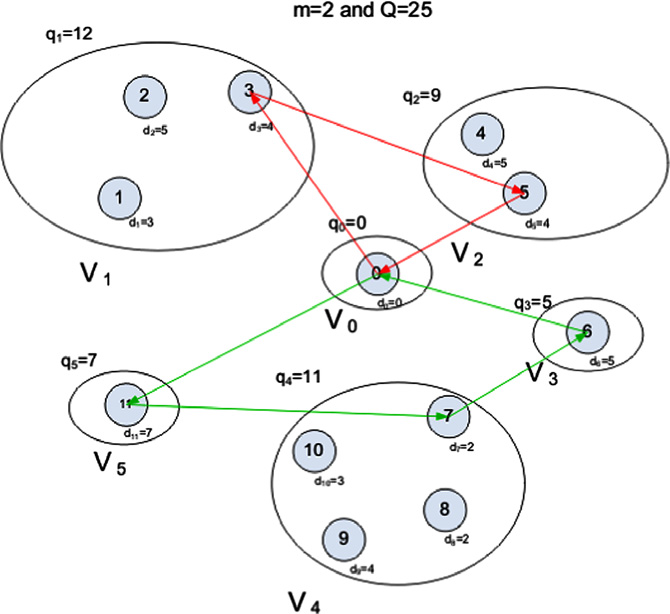
\includegraphics[width=0.6\textwidth]{example_gvrp.png}
\caption{An example of a GVRP and a feasible solution \citep{POP201297}}
\label{fig:example_gvrp}
\end{figure}

\section{MILP formulations}
The first mixed integer linear formulation of the GVRP was presented by \cite{bektasKara}, with a polynomially increasing number of binary variables and constraints. \cite{POP201297} presented two different formulations based on the additional auxiliary decision variables. These are called \emph{node-based} and \emph{flow-based} formulations respectively. The node-based formulation is structurally similar to the formulation by \cite{bektasKara}, but with stronger lower bounds. The flow-based formulation is completely new. In this section, a general semi-closed formulation for the GVRP is first presented and followed by the two formulations proposed by \cite{POP201297}.

\subsection{General formulation}
The related sets, decision variables and parameters for the GVRP are defined as follows:

\textit{Sets:}

$V = \{0,1,2,\ldots,n\}$ is the set of nodes corresponding to the customers, where 0 represents the depot. $V$ is partitioned into mutually exclusive and exhaustive non-empty sub-sets $V_0$, $V_1$, \ldots $V_k$, each of which represents a cluster of customers, where $V_0 = \{0\}$ is the depot.

$K = \{0,1,2,\ldots,k\}$ is the set of clusters.

$A = \{(i,j)|\; i,j\in V, i\ne j\}$ is the set of arcs.

\textit{Decision variables:}

We define the following binary variables:
\begin{flalign*}
    &x_{ij}= 
\begin{cases}
    1 & \text{if arc $(i,j)$ is included in the tour of a vehicle,  } i \in V_p, j \in V_r, p,r\in K, \\
    0,              & \text{otherwise}
\end{cases} \\
    &W_{pr}= 
\begin{cases}
    1 & \text{if there is a path from cluster $V_p$ to cluster $V_r$,  }  p,r\in K, \\
    0,              & \text{otherwise}
\end{cases}
\end{flalign*}

\textit{Parameters:}

$c_{ij}$ is the cost of traveling from node $i$ to node $j$, $i \ne j$, $i \in V_p$, $j \in V_r$, $p \ne r$, $p,r \in K$;

$d_i$ is the demand of customer $i$, $i = 1,2,\ldots ,n$;

$q_r$ is the demand of the cluster $V_r$, $q_r = \sum_{i \in V_r} d_i$, $r \in K$;

$M = \{1, \ldots,m\}$ is the set of identical vehicles;

$Q$ is the capacity of each vehicle.

We assume that $k \ge m$ ie. the number of vehicles is no greater than the number of clusters.

\subsubsection{Cluster degree constraints}
For each cluster except $V_0$, only a single outgoing arc to any other node belonging to other clusters can exist. This condition is expressed by:
\begin{equation}
\sum_{i \in V_p} \sum_{j\in V \backslash V_p} x_{ij} = 1, p \ne 0, p \in K
\label{cluster1}
\end{equation}
There can be exactly one incoming arc to a cluster from any other node belonging to other clusters, excluding $V_0$. This condition is implied by:
\begin{equation}
\sum_{i \in V \backslash V_p} \sum_{j\in V_p} x_{ij} = 1, p \ne 0, p \in K
\label{cluster2}
\end{equation}
There should be at most $m$ leaving arcs from and at most $m$ entering arcs to the depot:
\begin{flalign}
\sum_{i=1}^n x_{0 i} &\le m \label{cluster3}\\
\sum_{i=1}^n x_{i 0} &\le m \label{cluster4}
\end{flalign}
For the purposes of this study, the constraints \eqref{cluster3} \& \eqref{cluster4} have been taken to be equality constraints.
\subsubsection{Cluster connectivity constraints}
The entering and leaving nodes should be the same for each cluster, which is satisfied by:
\begin{equation}
\sum_{i \in V \backslash V_p} x_{ij} = \sum_{i \in V \backslash V_p} x_{ji}, j \in V_p, p \in K
\label{cluster5}
\end{equation}
Flows from cluster $V_p$ to the cluster $V_r$ are defined by $w_{pr}$. Thus, $w_{pr}$ should be equal to the sum of $x_{ij}$'s from $V_p$ to $V_r$:
\begin{equation}
w_{pr} = \sum_{i \in V_p} \sum_{j \in V_r} x_{ij}
\label{cluster6}
\end{equation}
With the above definitions and constraints, a general integer programming formulation for the GVRP is given as:
\begin{flalign}
\text{min} \; &\sum_{i=1}^n \sum_{j=1}^n c_{ij} x_{ij} \nonumber \\
\text{s.t.} \; & \text{\eqref{cluster1} - \eqref{cluster6}}  \nonumber \\
		  &\text{Capacity bounding constraints} \label{capbound} \\	
		  &\text{Subtour elimination constraints} \label{subtour}\\
		  &x_{i,j} \in \{0,1\}, \forall (i,j) \in A \nonumber
\end{flalign}

Integrality constraints do not need to be imposed on $w_{pr}$ because Eqs. \eqref{cluster1} - \eqref{cluster4} and \eqref{cluster6} automatically imply that $w_{pr}$ is either $0$ or $1$.

Model formulations of the GVRP are thus constrained by \eqref{cluster1} - \eqref{cluster6} and ``capacity bounding'' and ``subtour elimination'' constraints given in \eqref{capbound} and \eqref{subtour} above.

\subsection{Node-based formulation}
In this case, the additional auxiliary variables are defined with respect to the vertices of the graph:

$u_{p}$: the load of a vehicle just after leaving the cluster $V_p$, or delivered amount of goods just after leaving the cluster $V_p$, $p \ne 0$, $p \in K$.

\subsubsection{Capacity bounding constraints}
The capacity bounding constraints for the node-based formulation are given by:
\begin{align}
u_p - \sum_{r \in K, r \ne p}q_r w_{rp} \ge q_p, \; p \ne 0, p \in K \label{cbound1}\\
u_p + (Q - q_p) w_{0p} \le Q, \; p \ne 0, p \in K \label{cbound2}\\
u_p + \sum_{r \in K, r \ne p} q_r w_{pr} \le Q, \; p \ne 0, p \in K \label{cbound3}
\end{align}
\subsubsection{Subtour elimination constraints}
The formation of any subtour between clusters excluding $V_0$ will be prevented by the following constraint:
\begin{equation}
u_p - u_r + Q w_{pr} + (Q - q_p - q_r) w_{rp} \le Q - q_r, \;  p \ne r \ne 0; p, r \in K
\label{subtour1}
\end{equation}•
where $w_{pr} = 0$, whenever $q_p + q_r > Q$ with $p \ne r$ and $p, r \in K$. 

Hence the complete node based formulation is given by replacing Eqs. \eqref{capbound} and \eqref{subtour} in the generalized formulation by  Eqs. \eqref{cbound1} - \eqref{cbound3} and Eq. \eqref{subtour1} respectively.
%%%%%

\subsection{Flow-based formulation}
For the flow-based formulation, the additional auxiliary variables are defined with respect to the arcs of the graph:

$y_{pr}$: amount of goods picked up (or delivered in the case of delivery) on the route of a vehicle just after leaving the cluster $V_p$ if the vehicle goes from the cluster $V_p$ to the cluster $V_r$.
\subsubsection{Capacity bounding and subtour elimination constraints}
Capacity bounding and subtour elimination constraints for the flow-based formulation are given by:
\begin{align}
&y_{rp} \le (Q - q_p) w_{rp}, \; r \ne p; r,p \in K \label{flow1} \\
&y_{rp} \ge q_r w_{rp}, \;  r \ne p; r, p \in K \label{flow2}\\
&\sum_{p=1}^k y_{p0} =  \sum_{p=1}^k q_p \label{flow3} \\
&\sum_{p=0}^k y_{rp} - \sum_{p=0}^k y_{pr} = q_r, \; r \ne 0; r,p \in K \label{flow4}
\end{align}
where $y_{0p} = 0$ for all $p \in K$ and $q_0 = 0$.
Hence the complete flow based formulation is given by replacing Eqs. \eqref{capbound} and \eqref{subtour} in the generalized formulation by  Eqs. \eqref{flow1} - \eqref{flow4}.
\section{Test examples}
\begin{table}[htbp]
\centering
\caption{Details of GVRPs under consideration}
\label{tab:problemdetails}
\begin{tabular}{@{}cccccc@{}}
\toprule
\textbf{Instance} & \textbf{Customers} & \textbf{Clusters} & \textbf{Vehicles} & \textbf{Capacity} & \textbf{\begin{tabular}[c]{@{}c@{}}Total\\   demand\end{tabular}} \\ \midrule
\texttt{GVRP1}             & 50                 & 24                & 4                 & 15                & 50                                                                \\
\texttt{GVRP2}             & 60                 & 16                & 6                 & 15                & 60                                                                \\
\texttt{P-n50-k10}     & 49                 & 30                & 5                 & 200               & 951                                                               \\
\texttt{A-n69-k9}      & 68                 & 31                & 6                 & 150               & 845                                                               \\
\texttt{P-n76-k5}      & 75                 & 38                & 5                 & 280               & 1364                                                              \\ \bottomrule
\end{tabular}
\end{table}

Unfortunately, there are only two available test problems for the GVRP. The first, given by \cite{GHIANI200011} (denoted in this study by \texttt{GVRP1}), is originally a VRP taken from \cite{AraqueG1994} with 50 customers and 4 vehicles. Each customer has a unit demand and the demand of a cluster is equal to the cardinality of that cluster.

\cite{bektasKara} generated another test problem by clustering Problem 13 from \cite{AraqueG1994}. However, in the formulation under consideration in their work, an additional parameter $K$ is involved which is the minimum load of each vehicle when it returns to the depot (collection case) or minimum starting load of a vehicle just before starting its trip (delivery case). In this study, that parameter has not been considered while solving the instance. This particular problem is denoted by \texttt{GVRP2}. 

\subsection{Generation of additional test examples}

Three additional test examples were generated using capactitated vehicle routing problem (CVRP) data obtained from CVRPLIB (\url{http://vrp.atd-lab.inf.puc-rio.br}). Instances \texttt{P-n50-k10}, \texttt{A-n69-k9} and \texttt{P-n76-k5} were chosen. The clusters were obtained by implementation of a simple clustering algorithm (K-means), with the number of clusters chosen such that the number of customers in any cluster is no more than 5. The demand of each cluster was calculated by summing the demands of each customer in that cluster. 
Details of each of the problems under consideration is given in Table \ref{tab:problemdetails}.

\section{Computational study}

Both node-based and flow-based formulations described above were implemented in CPLEX and solved using a Windows PC with an Intel i7 processor (2.90 GHz). 

\subsection{Tightness of root node relaxation}

\begin{table}[htbp]
\centering
\caption{Deviation between root node relaxation and optimal values}
\label{tab:rootnode}
\begin{tabular}{@{}ccccc@{}}
\toprule
\textbf{Instance}              & \textbf{\begin{tabular}[c]{@{}c@{}}Best known\\  objective\end{tabular}} & \textbf{Formulation} & \textbf{\begin{tabular}[c]{@{}c@{}}Root node\\   relaxation\end{tabular}} & \textbf{\% Deviation} \\ \midrule
\multirow{2}{*}{\texttt{GVRP1}}          & \multirow{2}{*}{527.813}     & flow                 & 498.594                        & 5.54                  \\
                               &                              & node                 & 449.358                       & 14.86                 \\ \midrule
\multirow{2}{*}{\texttt{GVRP2}}         & \multirow{2}{*}{557.564}     & flow                 & 533.9                       & 4.24                  \\
                               &                              & node                 & 545.365                       & 2.19                  \\ \midrule
\multirow{2}{*}{\texttt{P-n50-k10}} & \multirow{2}{*}{417.742}     & flow                 & 384.597  & 7.93                  \\
                               &                              & node                 & 338.098                       & 19.07	  \\ \midrule
\multirow{2}{*}{\texttt{A-n69-k9}}  & \multirow{2}{*}{756.131}     & flow                 & 692.212 & 8.45                  \\
                               &                              & node                 & 560.44                       & 25.88 \\ \midrule
\multirow{2}{*}{\texttt{P-n76-k5}}  & \multirow{2}{*}{500.955}     & flow                 & 450.746                       & 11.27                 \\
                               &                              & node                 & 399.788                        & 21.30                 \\ \bottomrule
\end{tabular}
\end{table}

Table \ref{tab:rootnode} shows a comparision between the root node relaxations for the flow- and node-based formulations. In all but one of the instances under consideration, the flow-based formulation shows a tighter LP lower bound. Thus we would expect the flow-based formulation to be more efficient than the node-based formulation. 

This is indeed the case as seen in Table \ref{tab:compstudy}: the flow-based formulation finds a better objective value or closes the relative gap more than the node-based formulation. A one hour time limit for each problem was set for each of these calculations. Both formulations found the proven optimum within the time limit only for \texttt{GVRP2}. For \texttt{GVRP1}, only the flow-based formulation reached zero gap in 85 seconds. In all the other instances, the realtive gap at time limit was significantly smaller for the flow-based formulation.

\begin{table}[htbp]
\centering
\caption{Model comparision for GVRP instances (time limit = 1 hour)}
\label{tab:compstudy}
\begin{tabular}{@{}cccccc@{}}
\toprule
\textbf{Instance}              & \textbf{Formulation} & \textbf{Status} & \textbf{\begin{tabular}[c]{@{}c@{}}Objective\\   value\end{tabular}} & \textbf{\begin{tabular}[c]{@{}c@{}}Relative gap\\   (\%)\end{tabular}} & \textbf{\begin{tabular}[c]{@{}c@{}}Number \\ of constraints\end{tabular}} \\ \midrule
\multirow{2}{*}{\texttt{GVRP1}}         & flow                 & Optimal         & 527.813            & 0.01                       & 2108                 \\
                               & node                 & Feasible        & 527.813            & 5.42                       & 1482                 \\ \midrule
\multirow{2}{*}{\texttt{GVRP2}}         & flow                 & Optimal         & 557.564            & 0.00                       & 1242                 \\
                               & node                 & Optimal         & 557.564            & 0.00                       & 952                  \\ \midrule
\multirow{2}{*}{\texttt{P-n50-k10}} & flow                 & Feasible        & 417.742            & 0.75                       & 3094                 \\
                               & node                 & Feasible        & 417.742            & 14.69                      & 2132                 \\ \midrule
\multirow{2}{*}{\texttt{A-n69-k9}}  & flow                 & Feasible        & 756.131            & 1.25                       & 3385                 \\
                               & node                 & Feasible        & 763.045            & 18.59                      & 2360                 \\ \midrule
\multirow{2}{*}{\texttt{P-n76-k5}}  & flow                 & Feasible        & 508.194            & 6.04                       & 4896                 \\
                               & node                 & Feasible        & 595.149            & 31.20                      & 3374                 \\ \bottomrule
\end{tabular}
\end{table}

\begin{figure}[htbp]
\centering
\subfloat[Customer clusters]{%
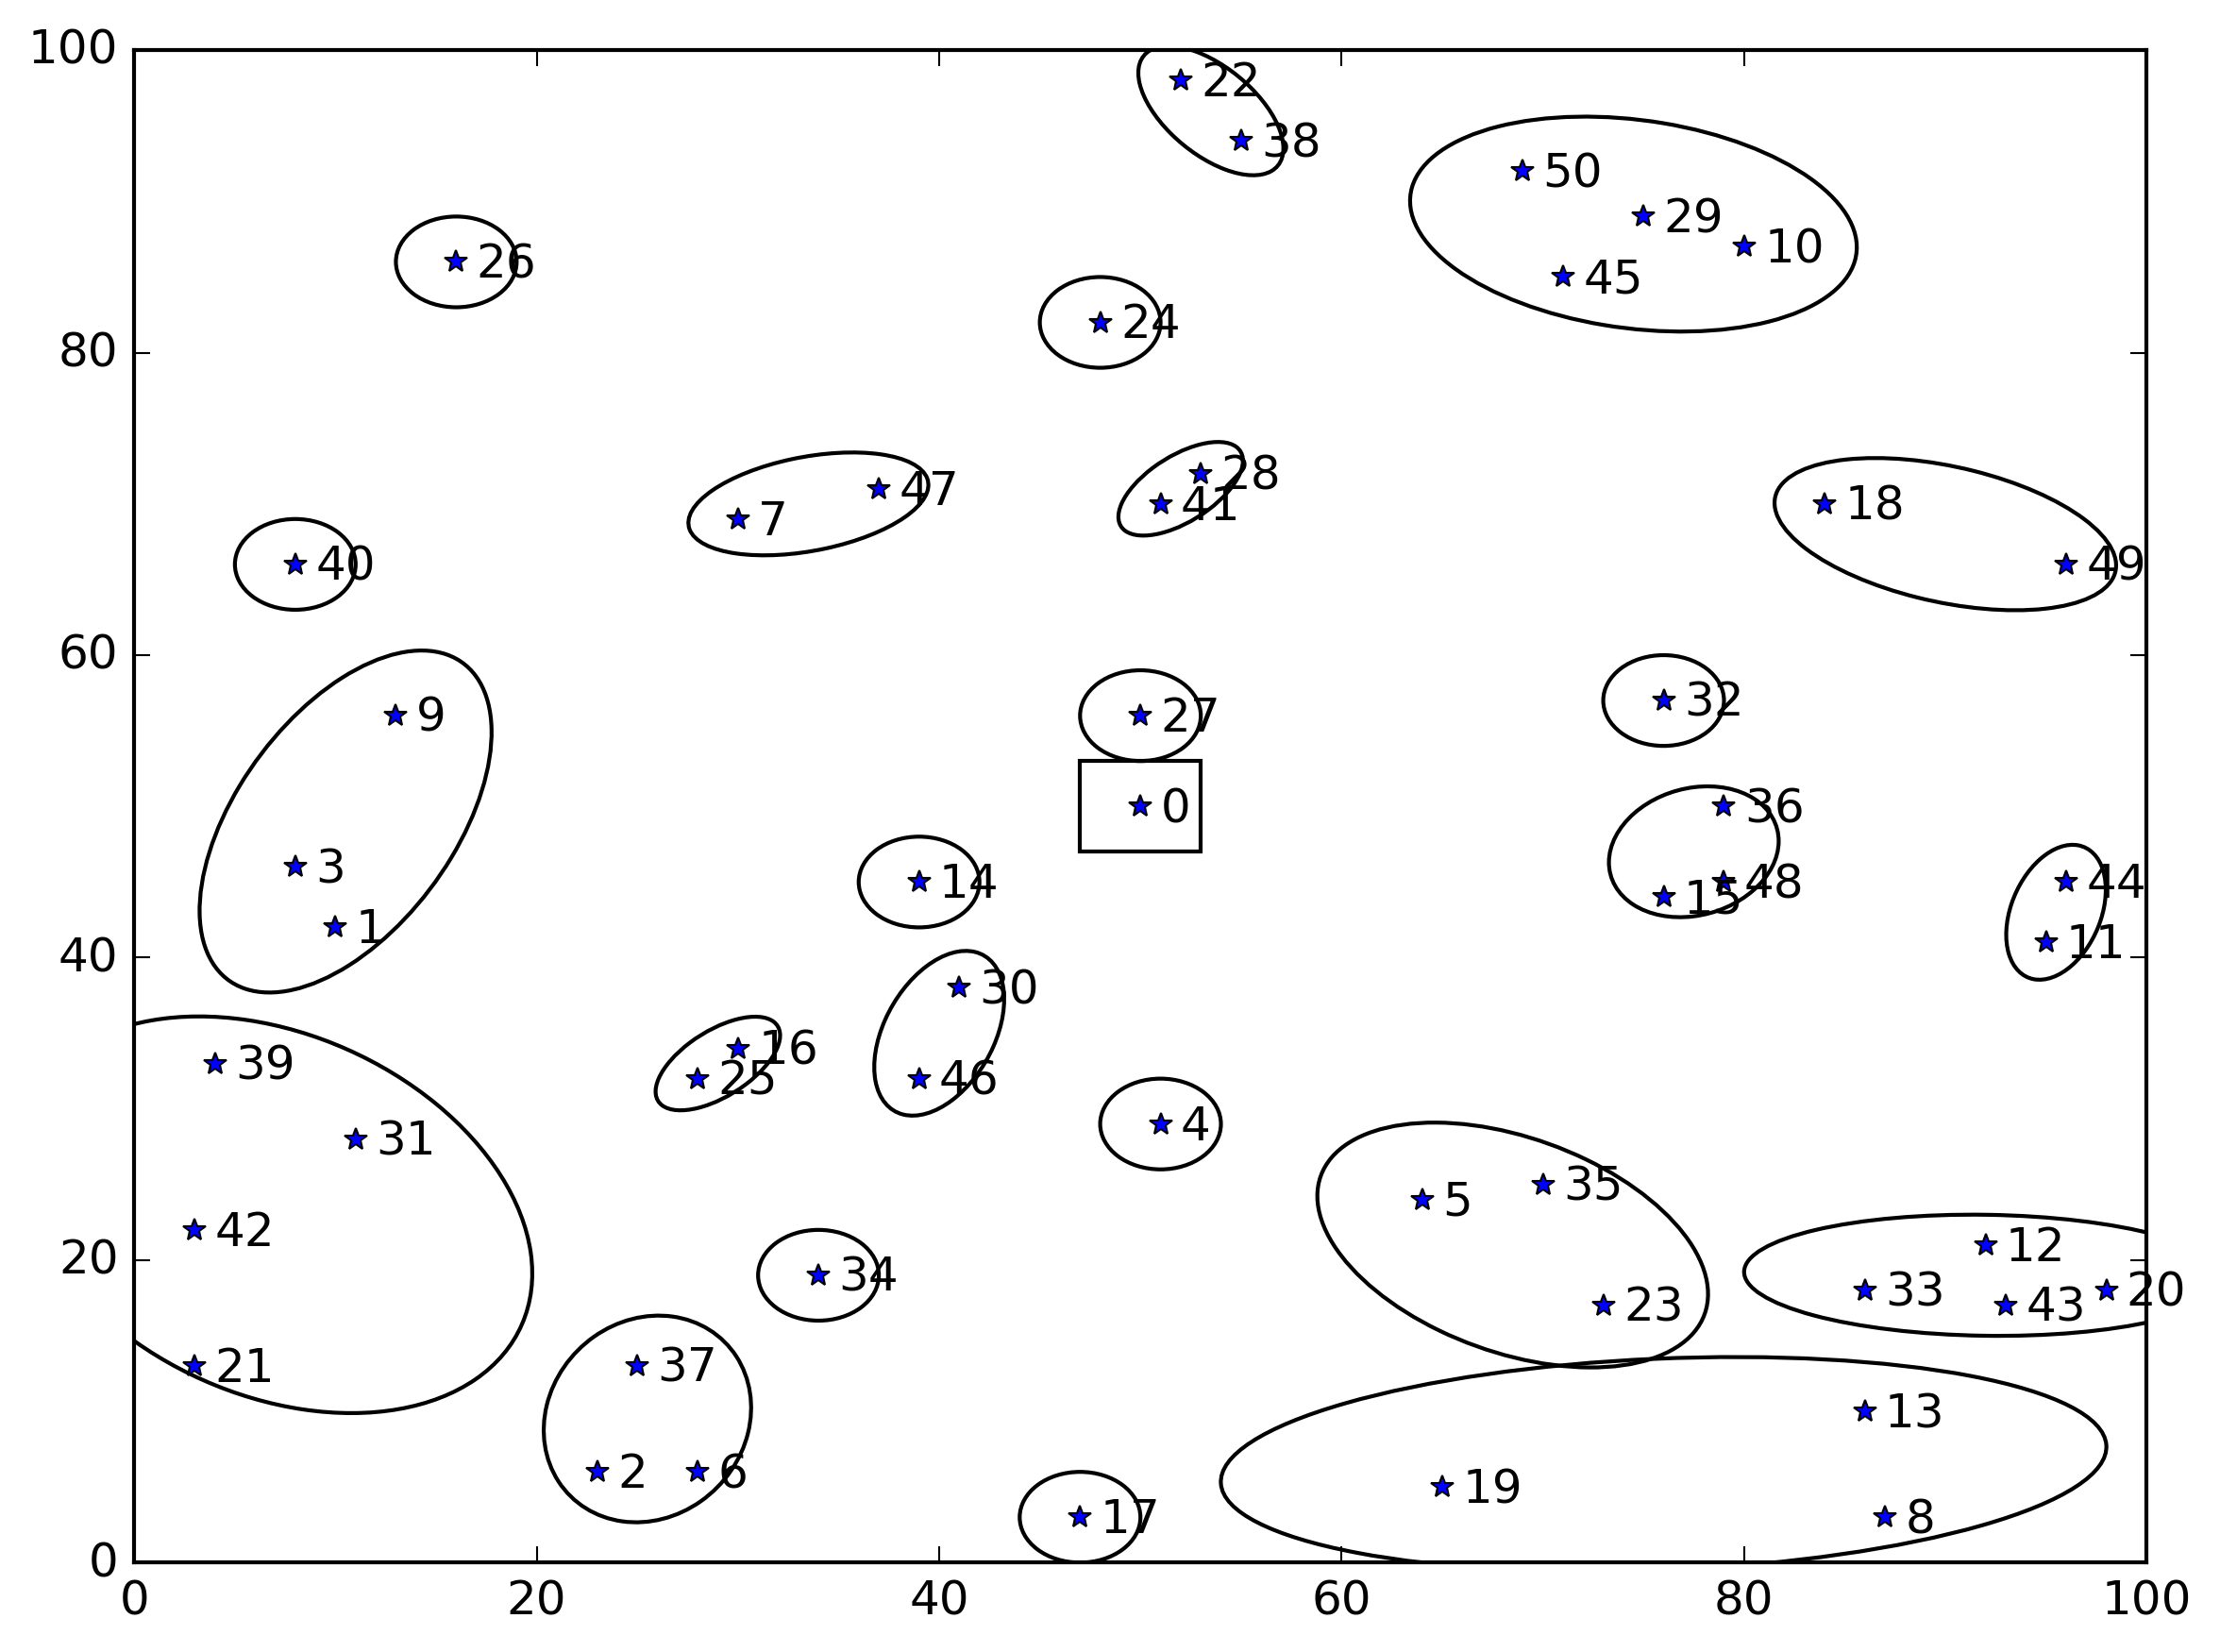
\includegraphics[width=0.45\textwidth]{GVRP_map.png}
\label{fig:plot_11}}
\quad
\subfloat[Optimum solution (objective = 527.813)]{%
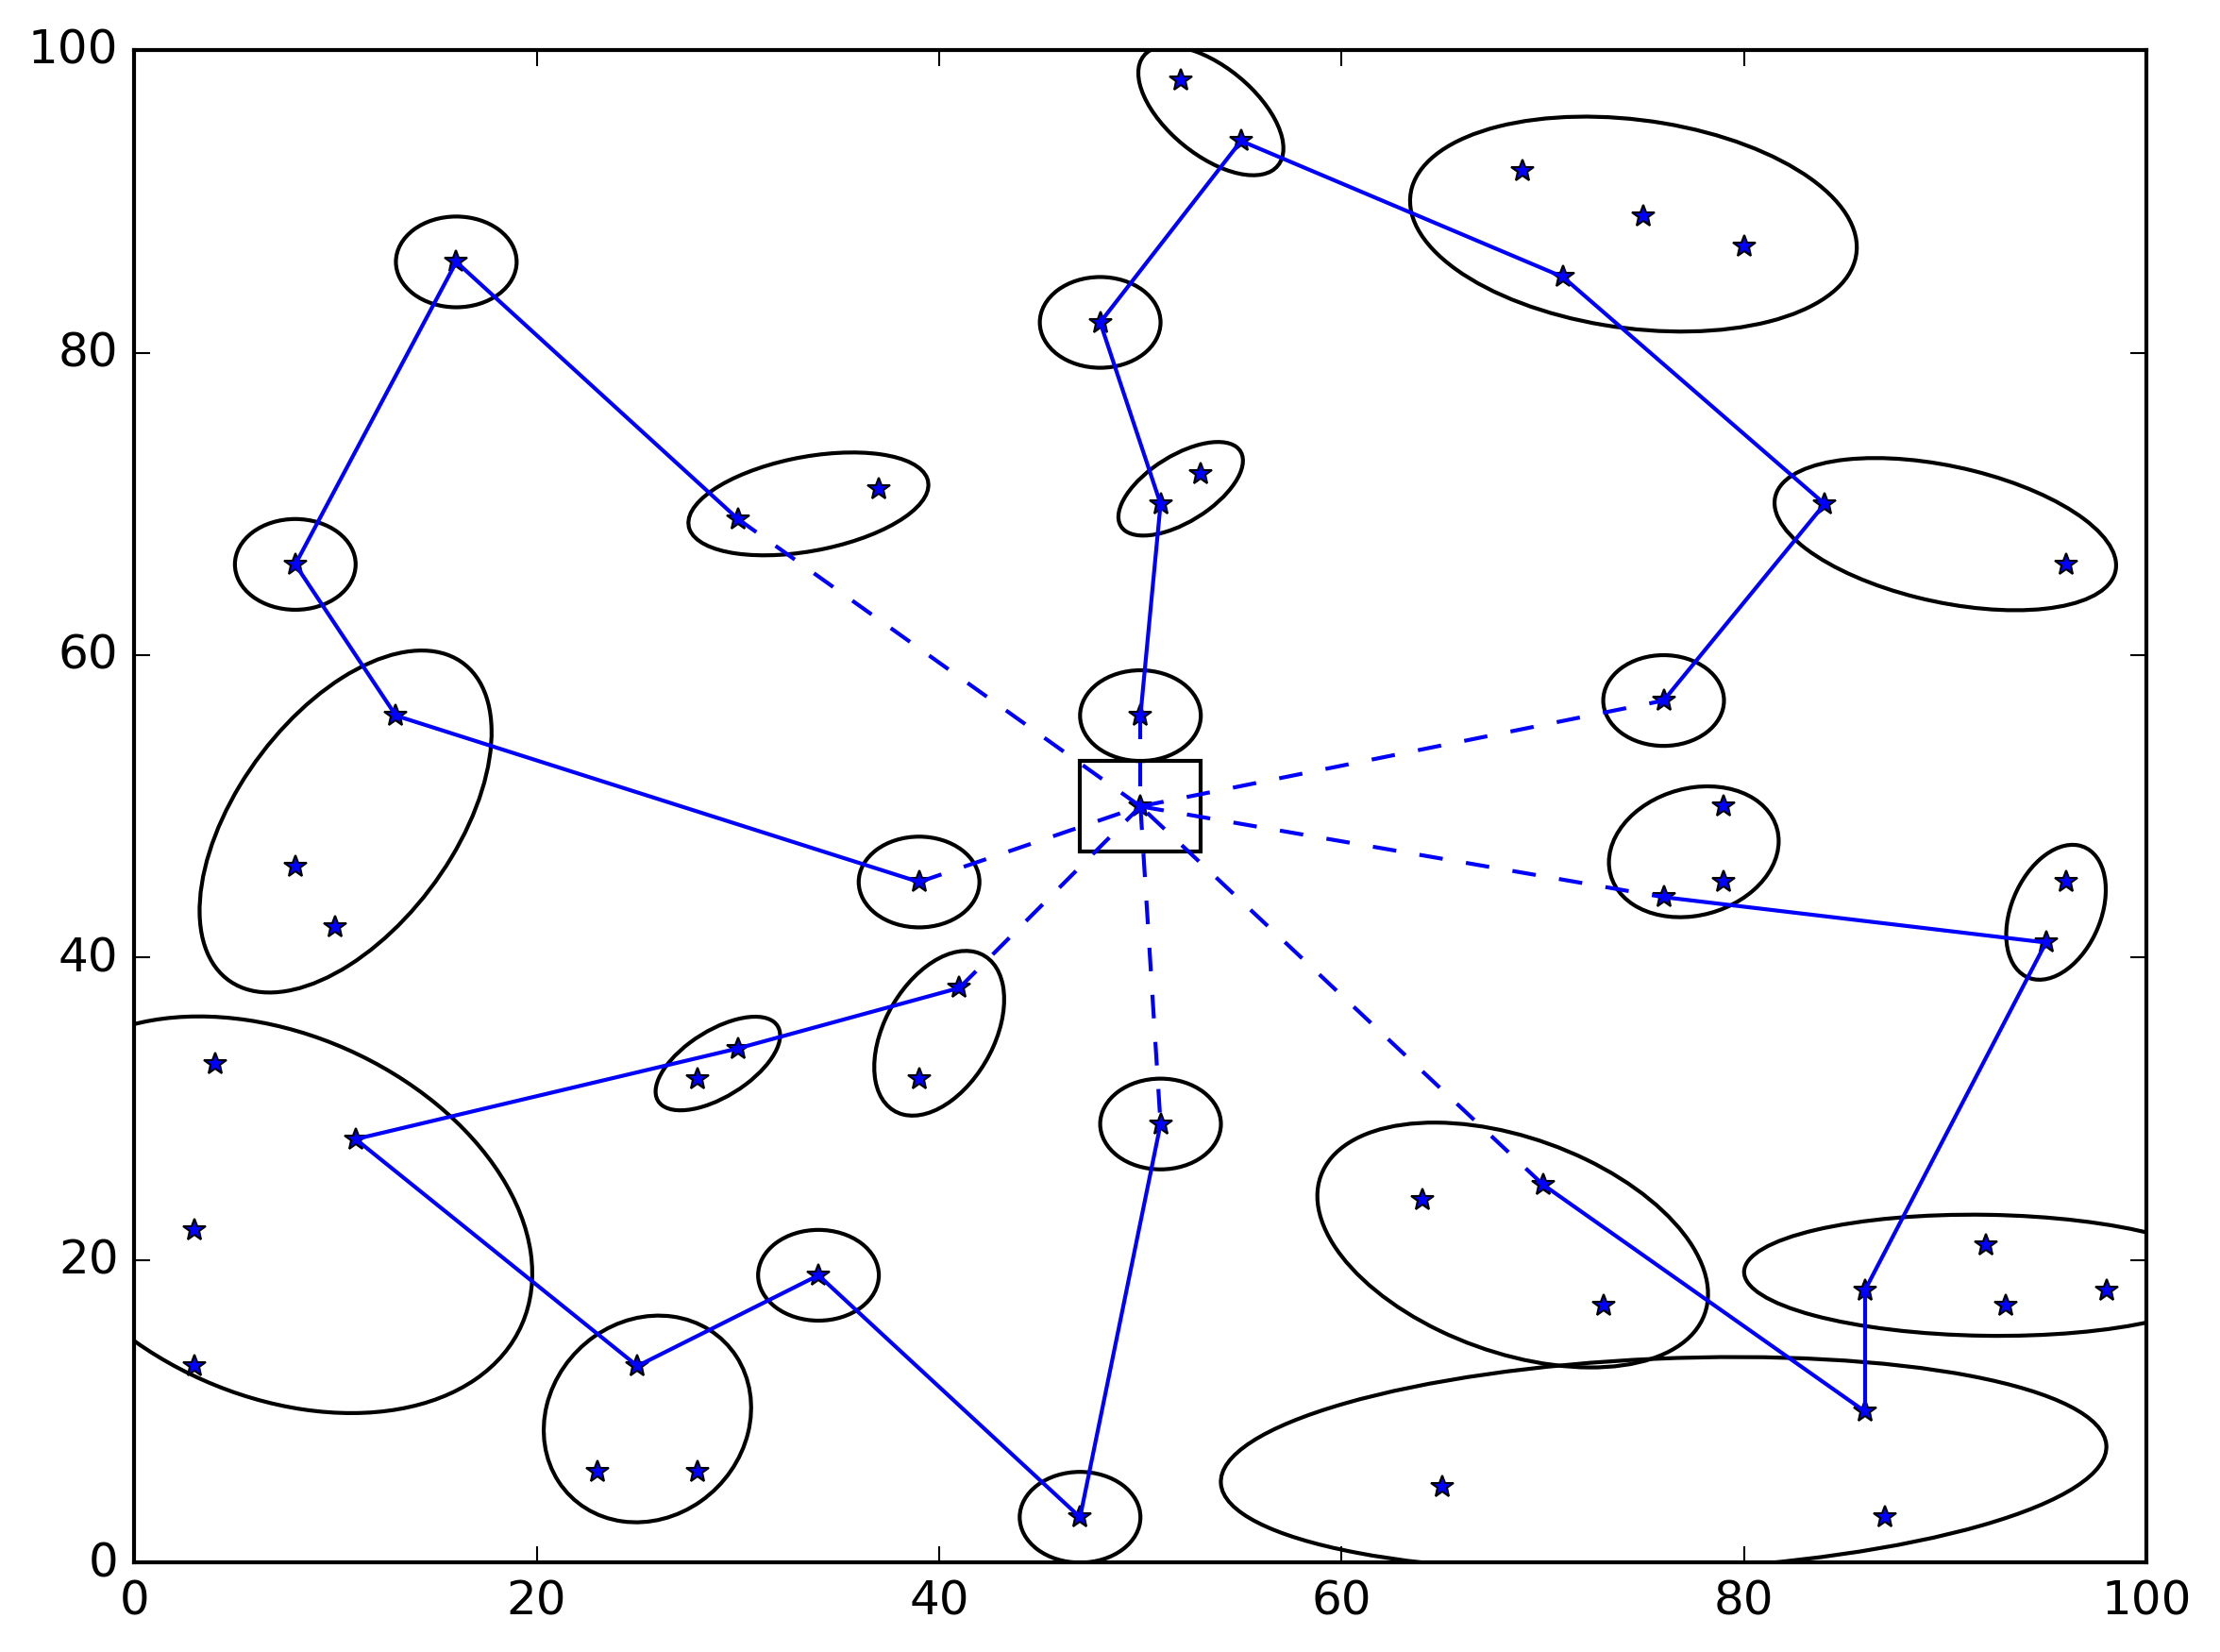
\includegraphics[width=0.45\textwidth]{GVRP_flow_n51_k25_m4_Q15_TL60_map.png}
\label{fig:plots_12}}
\caption{\texttt{GVRP1}}
\label{fig:GVRP1sol}
\end{figure}

\begin{figure}[htbp]
\centering
\subfloat[Customer clusters]{%
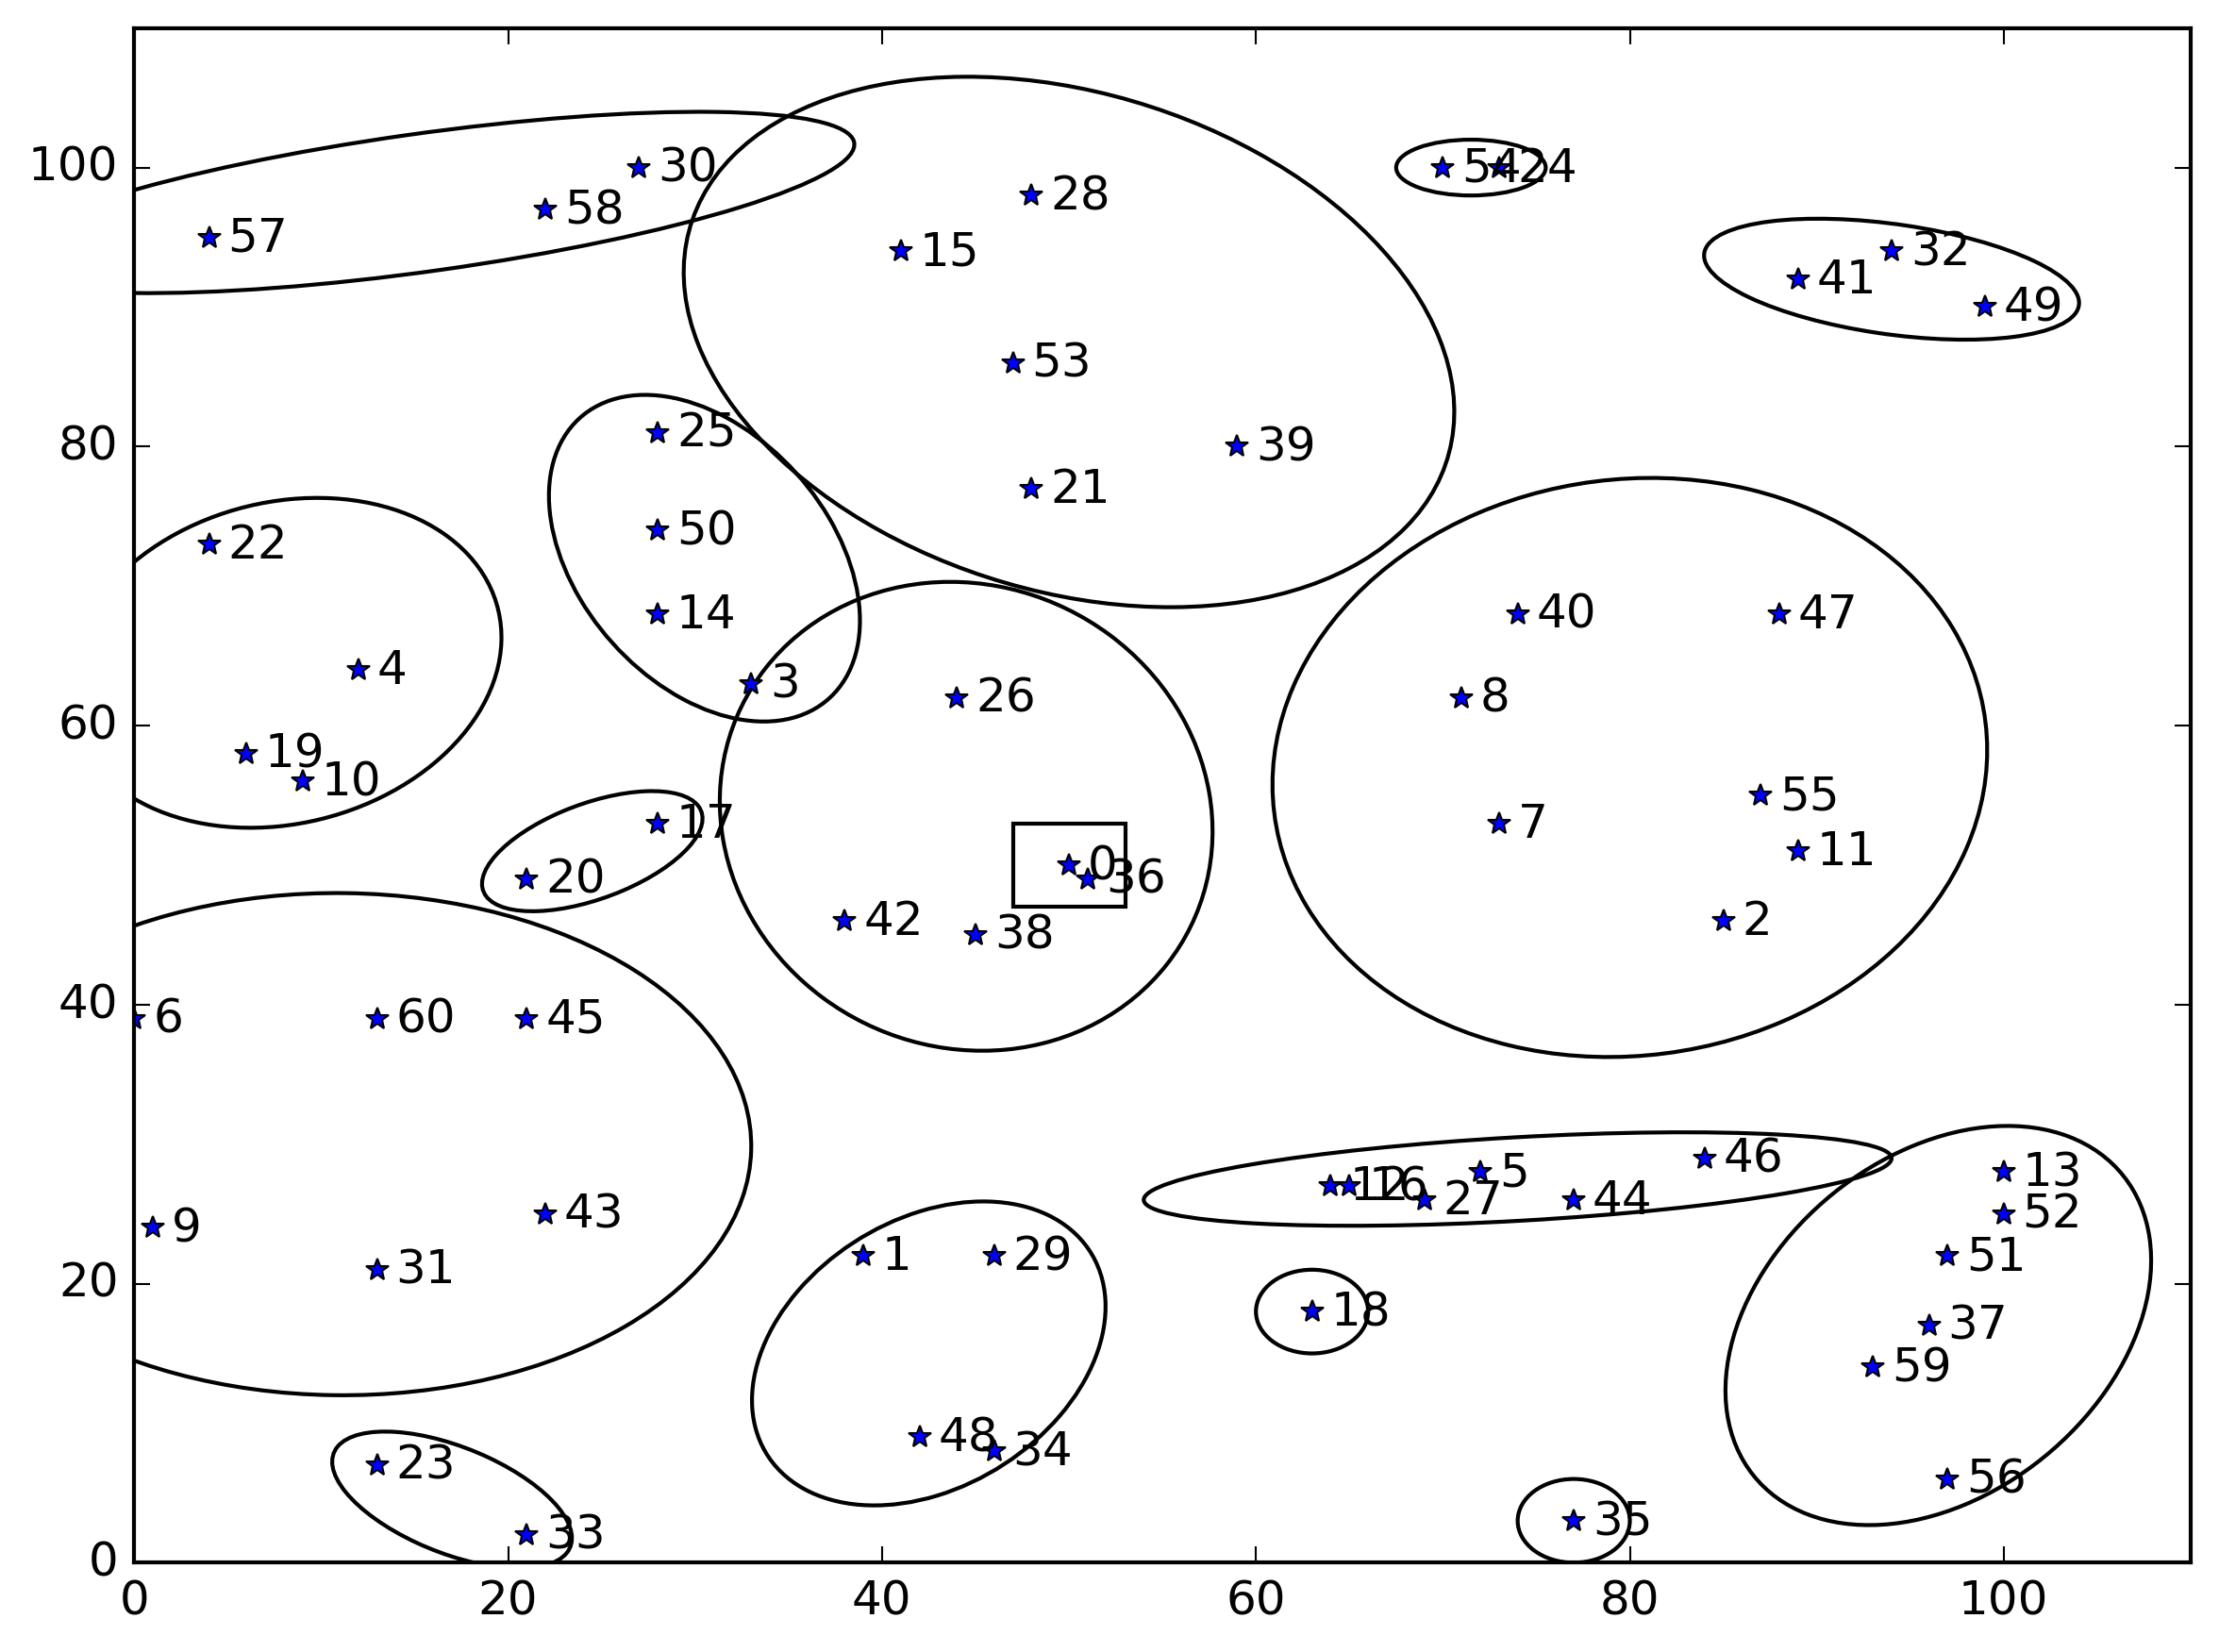
\includegraphics[width=0.45\textwidth]{GVRP2_map.png}
\label{fig:plot_11}}
\quad
\subfloat[Optimal solution (objective = 557.564)]{%
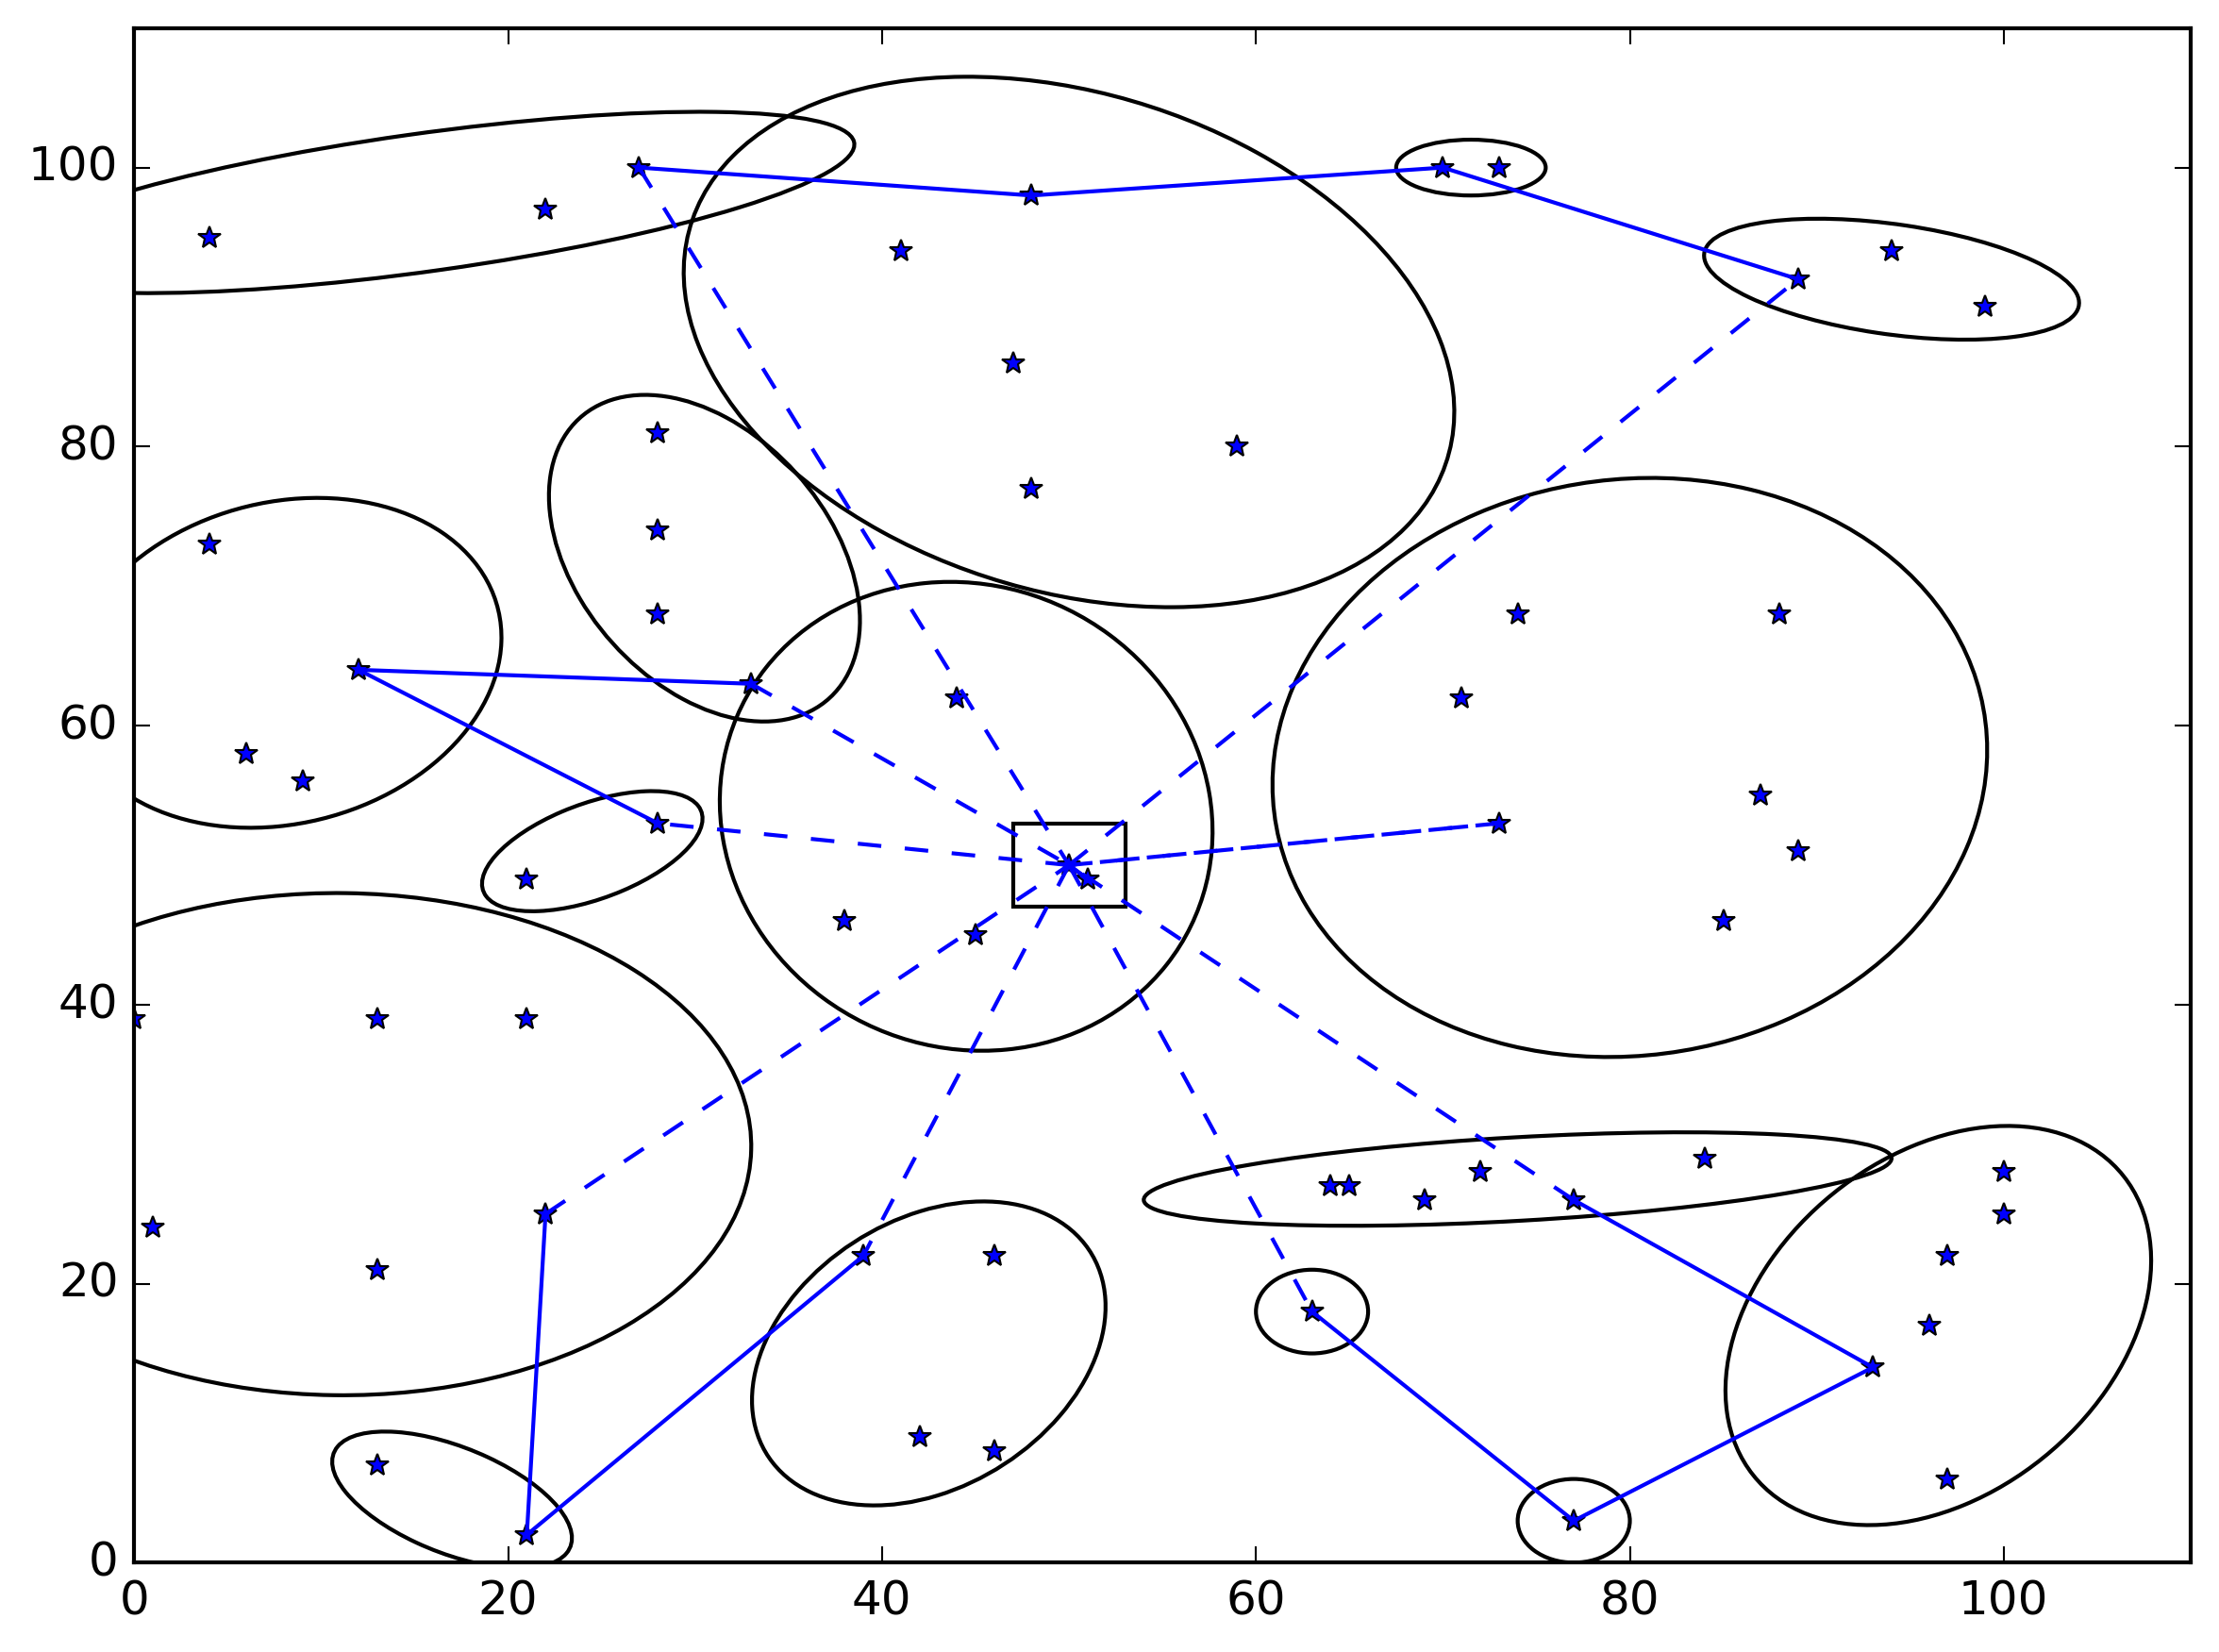
\includegraphics[width=0.45\textwidth]{GVRP2_flow_n61_k17_m6_Q15_TL10_map.png}
\label{fig:plots_12}}
\caption{\texttt{GVRP2}}
\label{fig:GVRP2sol}
\end{figure}
The obtained objective value for \texttt{GVRP1} (Fig. \ref{fig:GVRP1sol}) is the same as the optimum reported by \cite{POP201297}. Since different constraints were used for \texttt{GVRP2}, the obtained solution does not match that reported by \cite{bektasKara}.

Instances \texttt{P-n50-k10} and \texttt{A-n69-k9}, were solved to optimality with the flow-based formulation in 4100 s and 9120 s respectively. The instances and obtained solutions are shown in Fig. \ref{fig:P-n50-k10-sol} and \ref{fig:A-n69-k9-sol} respectively. Instance \texttt{P-n76-k5} was solved to 2.55\% relative gap with an 8 hour time limit. The solution is shown in Fig. \ref{fig:P-n76-k5-c38-sol }.

\begin{figure}[htbp]
\centering
\subfloat[Customer clusters]{%
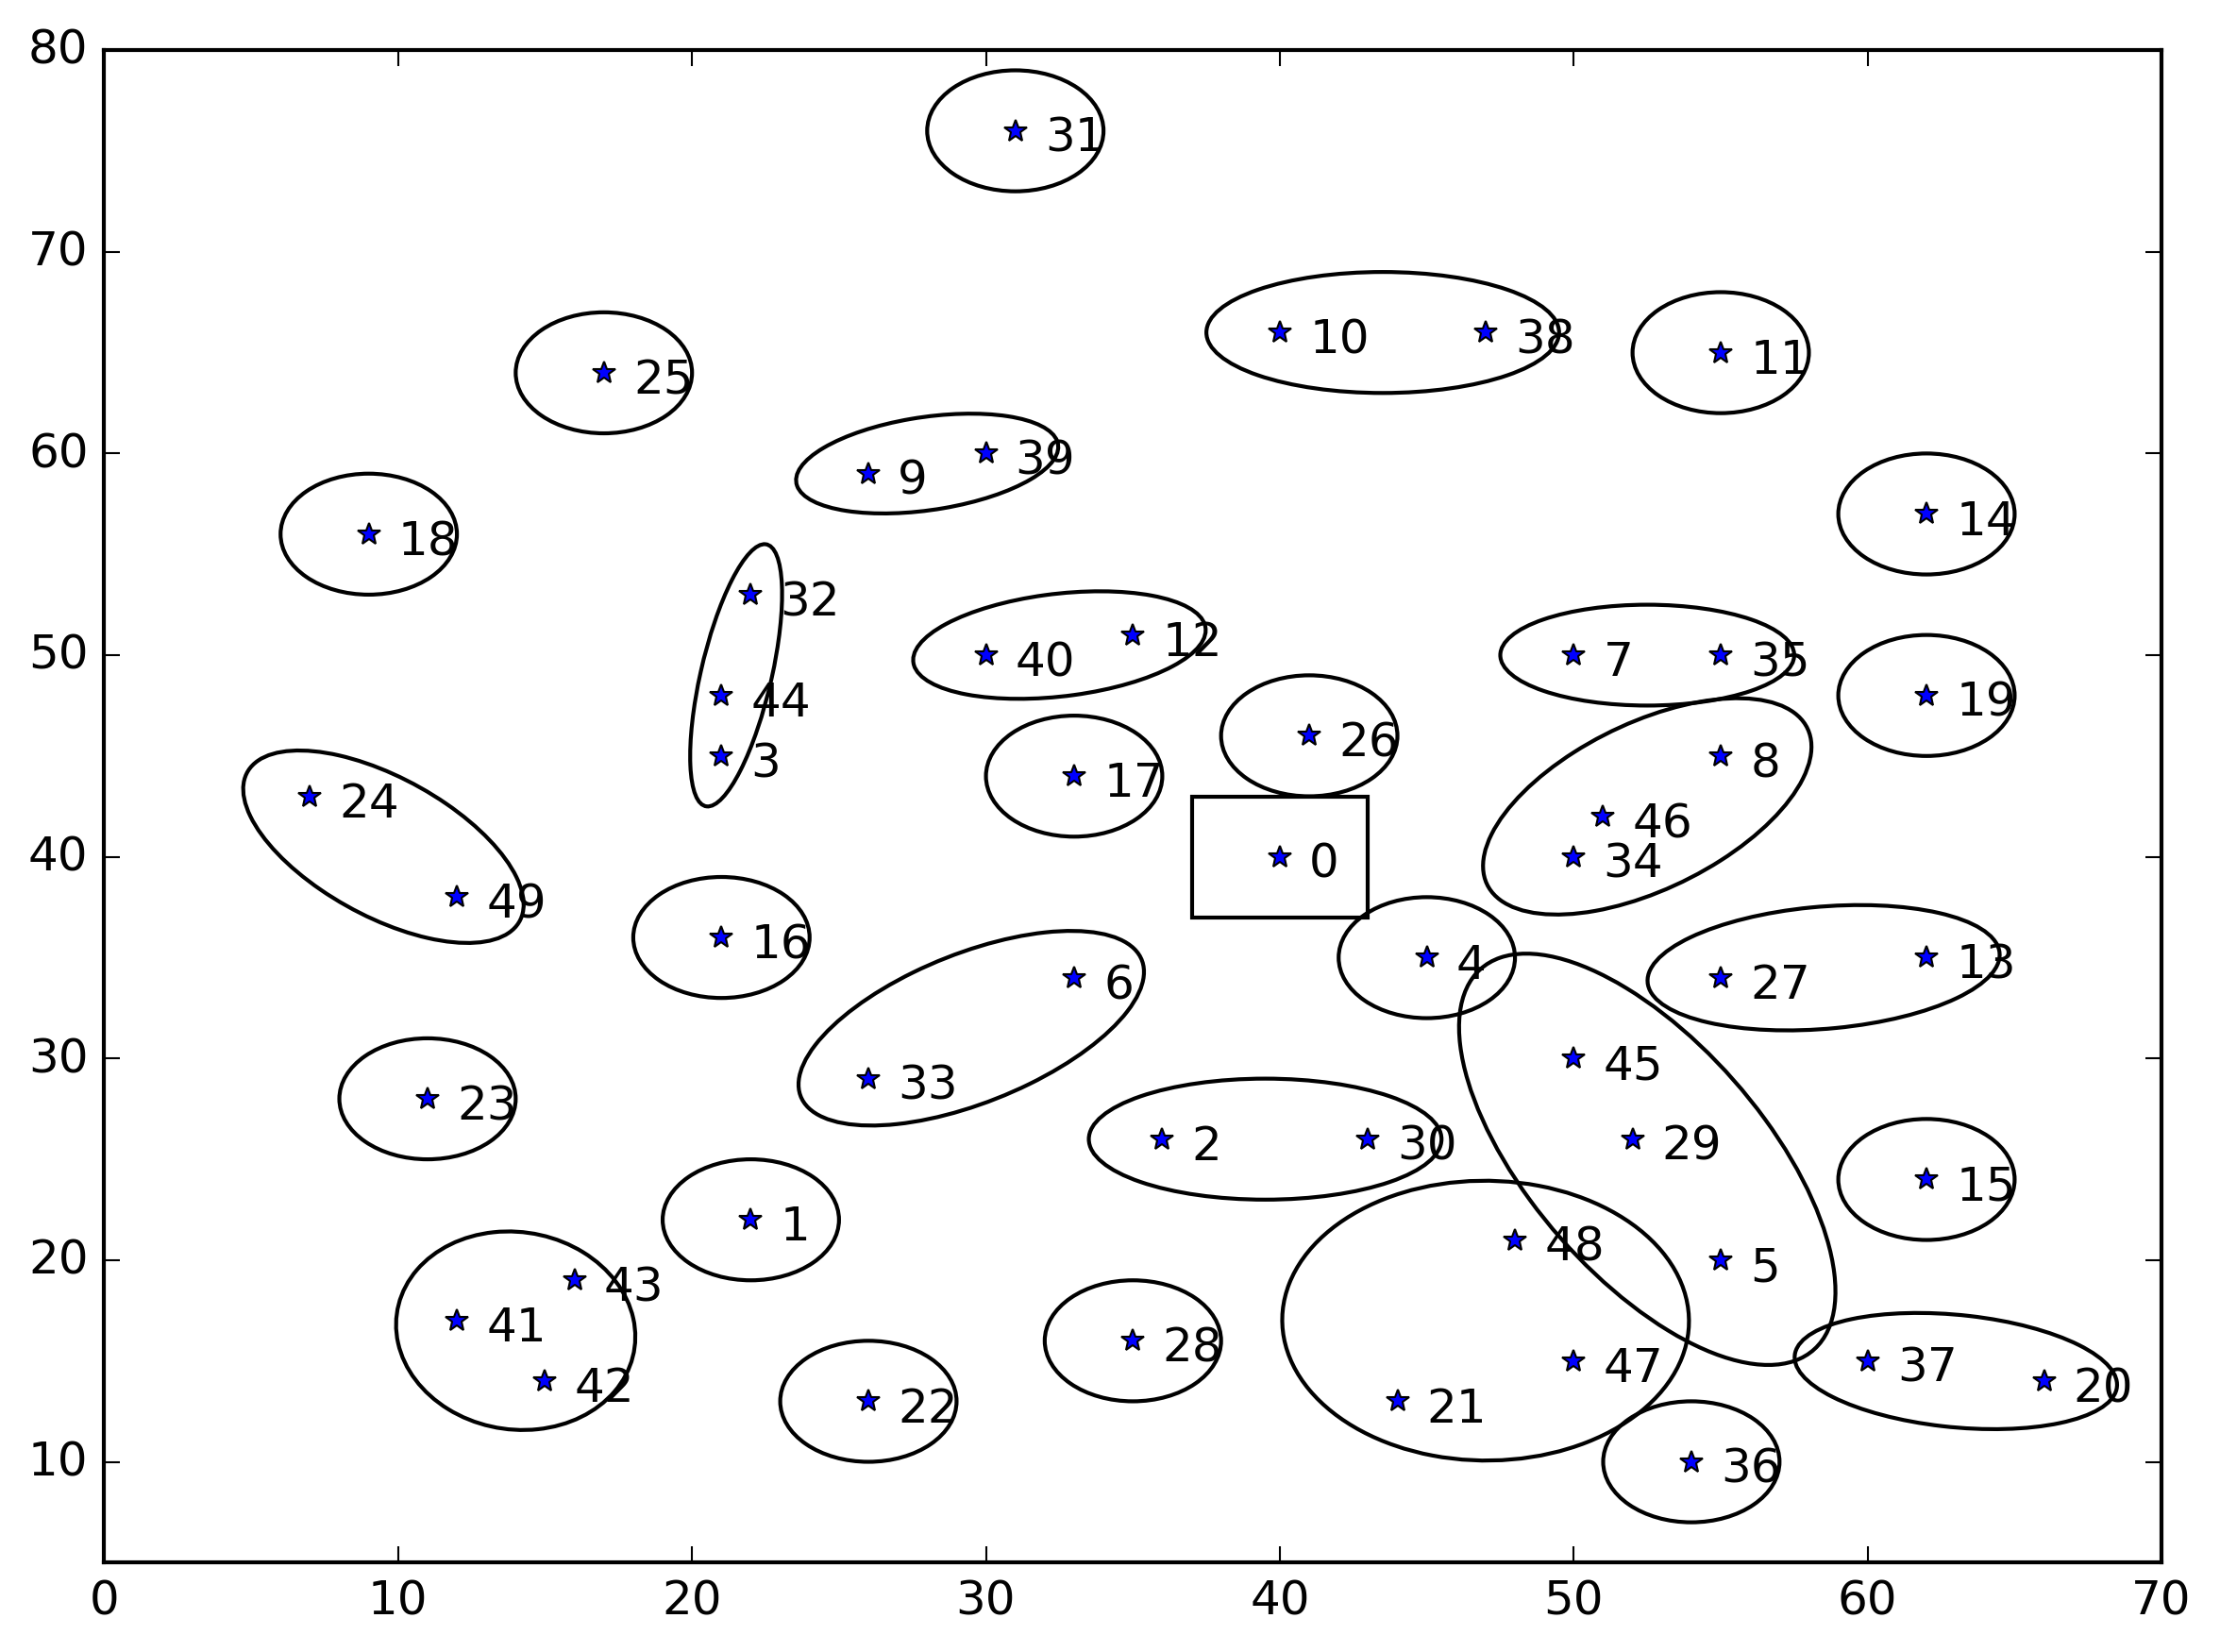
\includegraphics[width=0.45\textwidth]{P-n50-k10-c30_map.png}
\label{fig:plot_11}}
\quad
\subfloat[Optimal solution (objective = 417.742)]{%
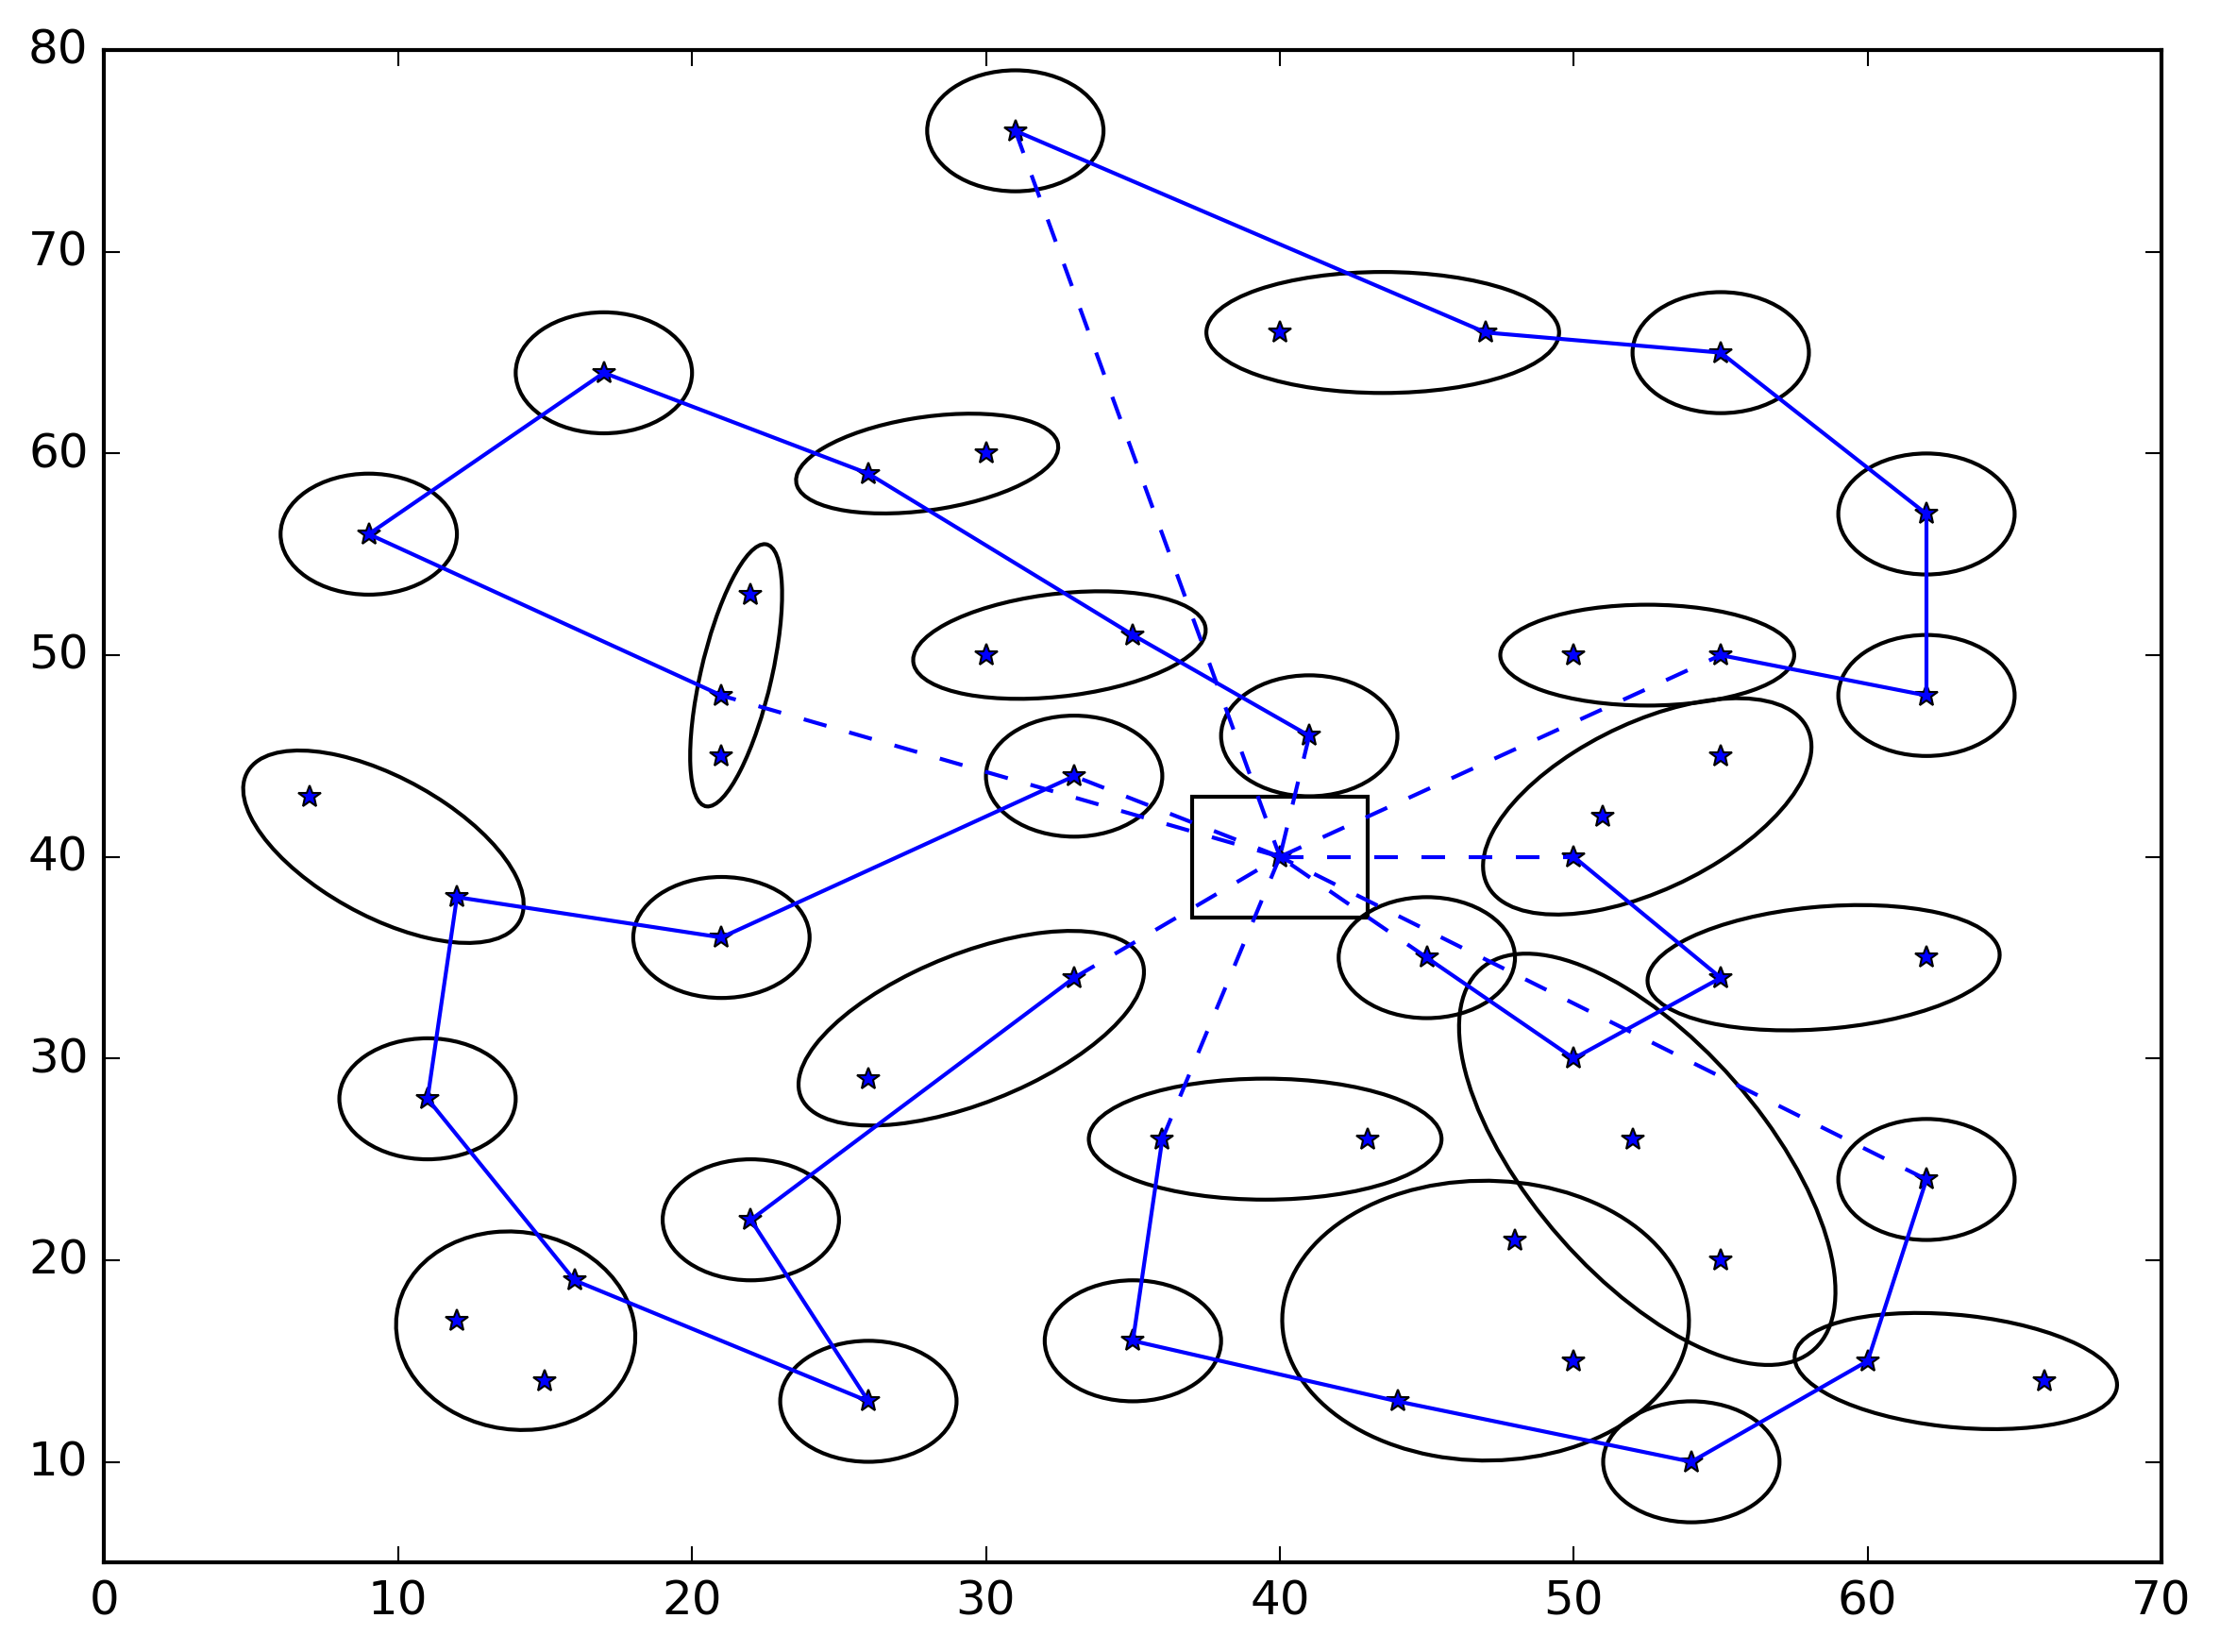
\includegraphics[width=0.45\textwidth]{P-n50-k10-c30_flow_n50_k31_m5_Q200_TL150_optimum.png}
\label{fig:plots_12}}
\caption{\texttt{P-n50-k10} (clustered)}
\label{fig:P-n50-k10-sol}
\end{figure}

\begin{figure}[htbp]
\centering
\subfloat[Customer clusters]{%
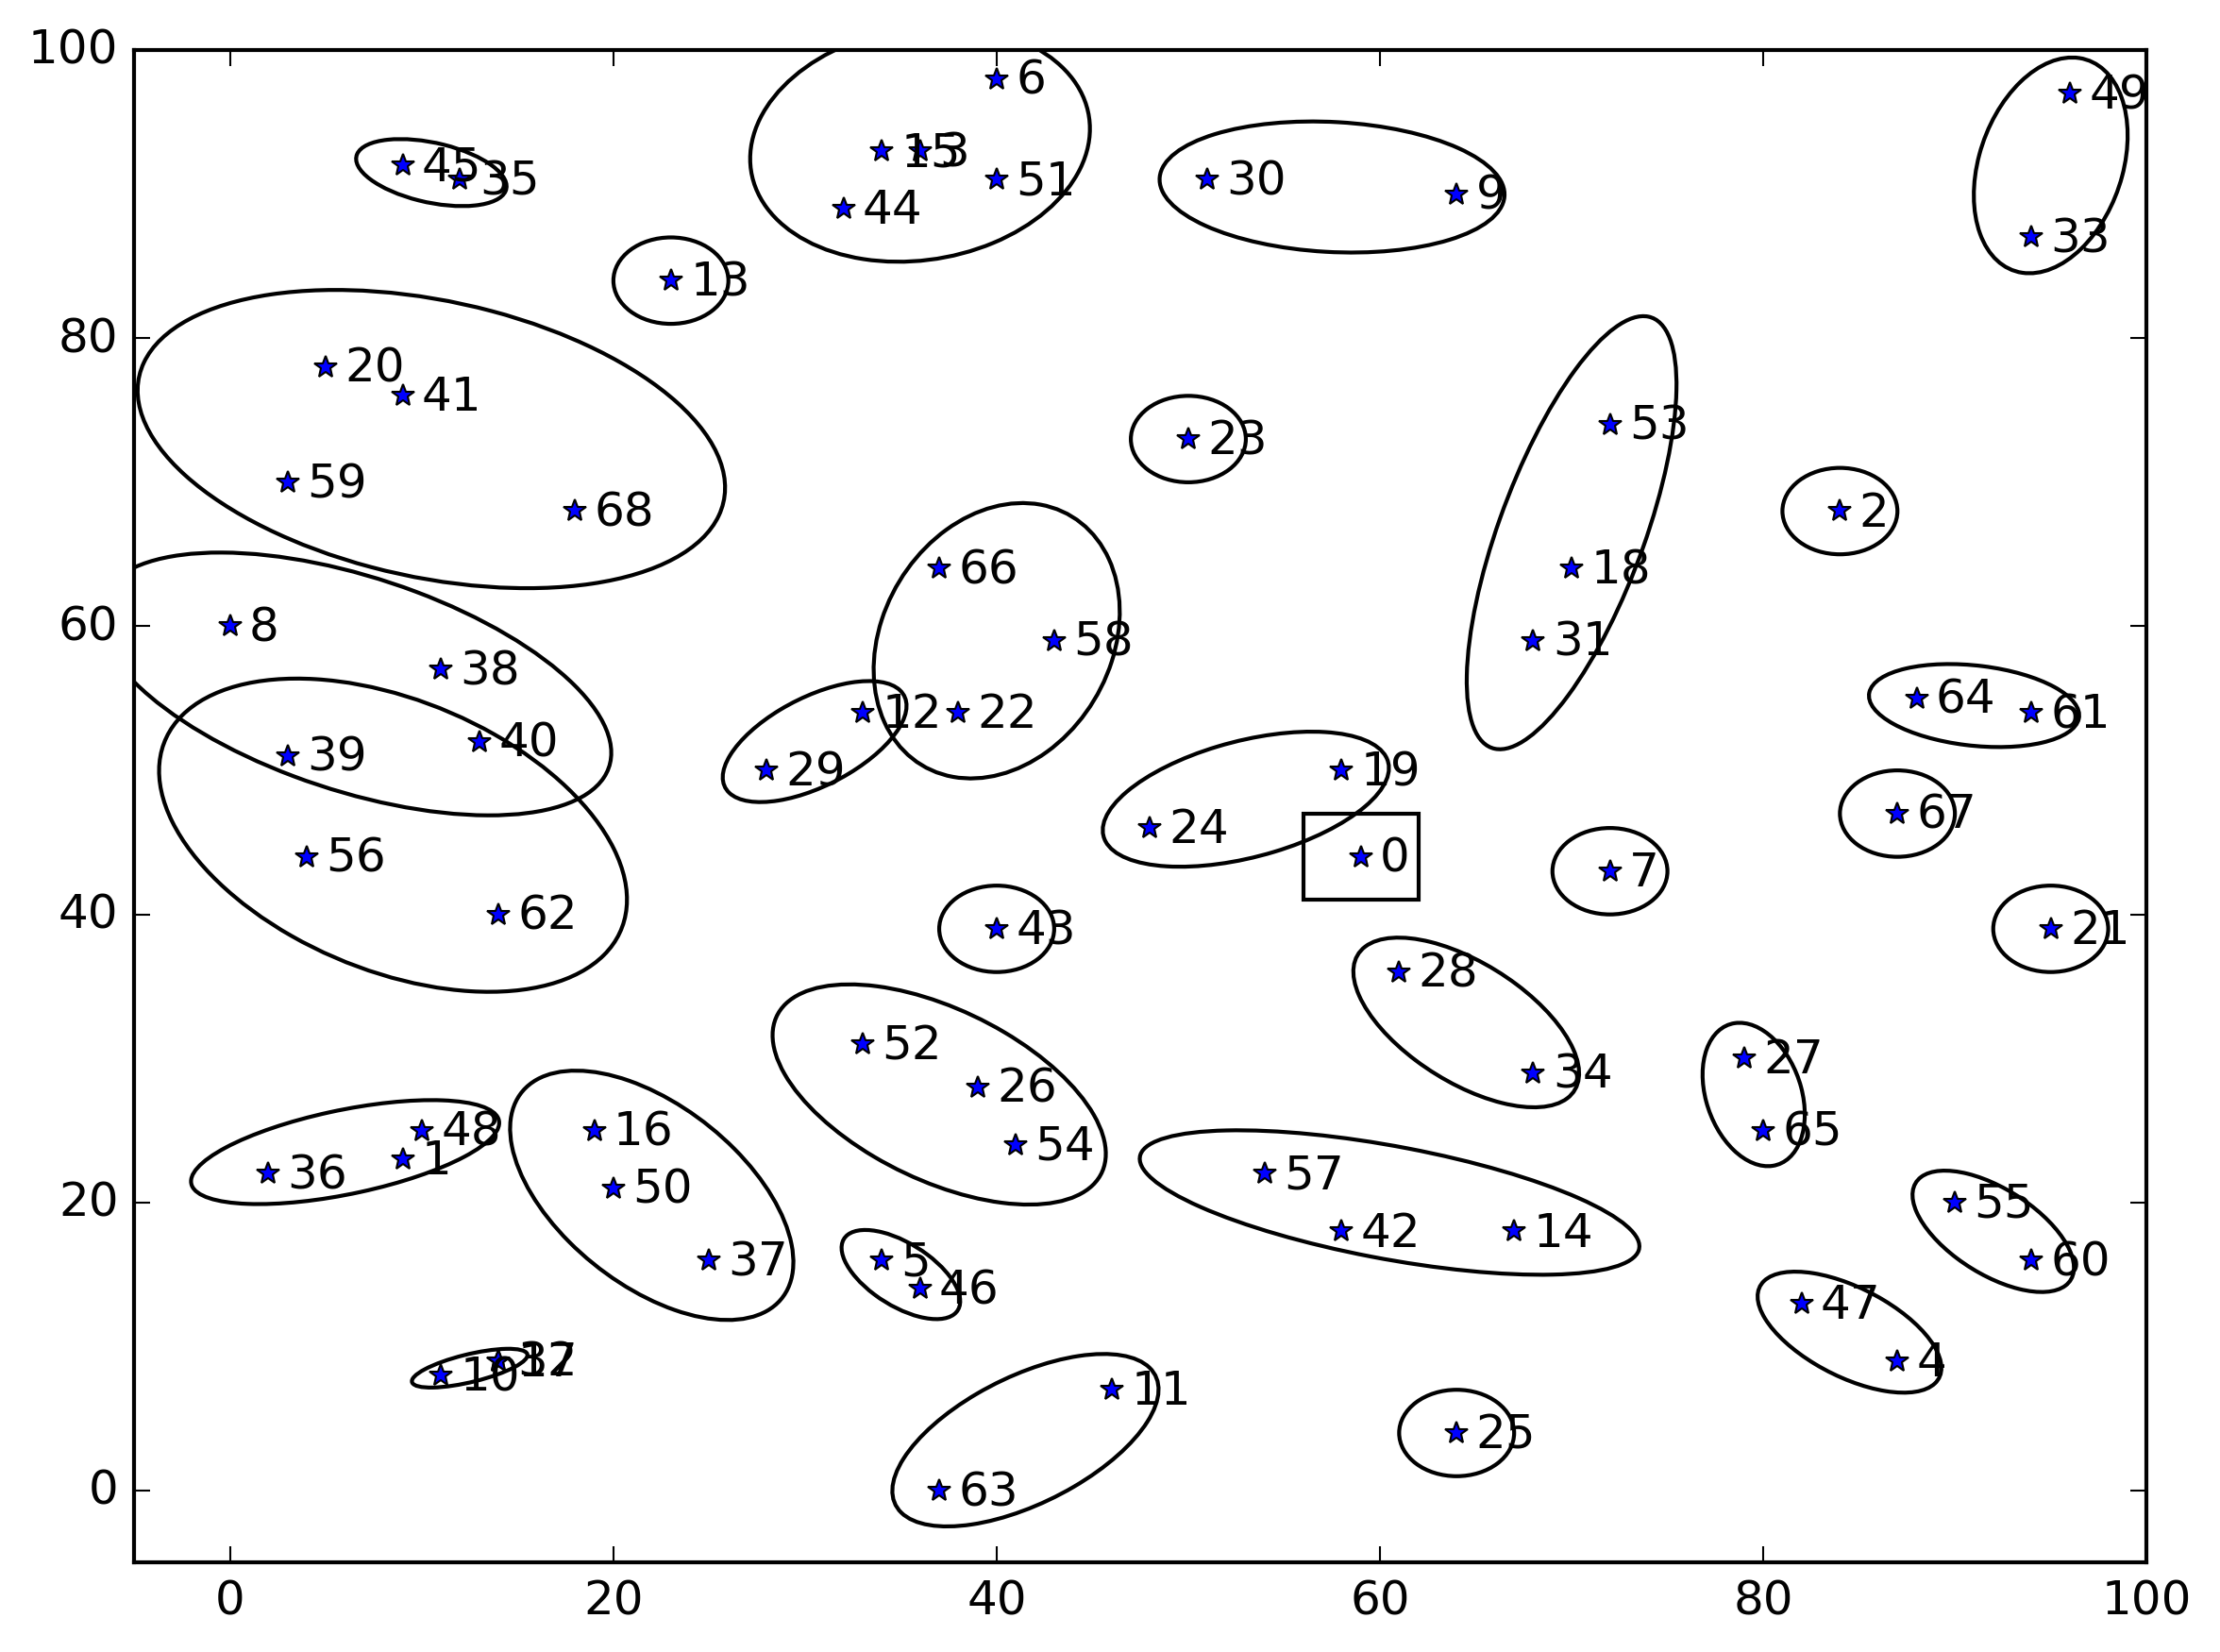
\includegraphics[width=0.45\textwidth]{A-n69-k9-c31_map.png}
\label{fig:plot_11}}
\quad
\subfloat[Optimal solution (objective = 756.131)]{%
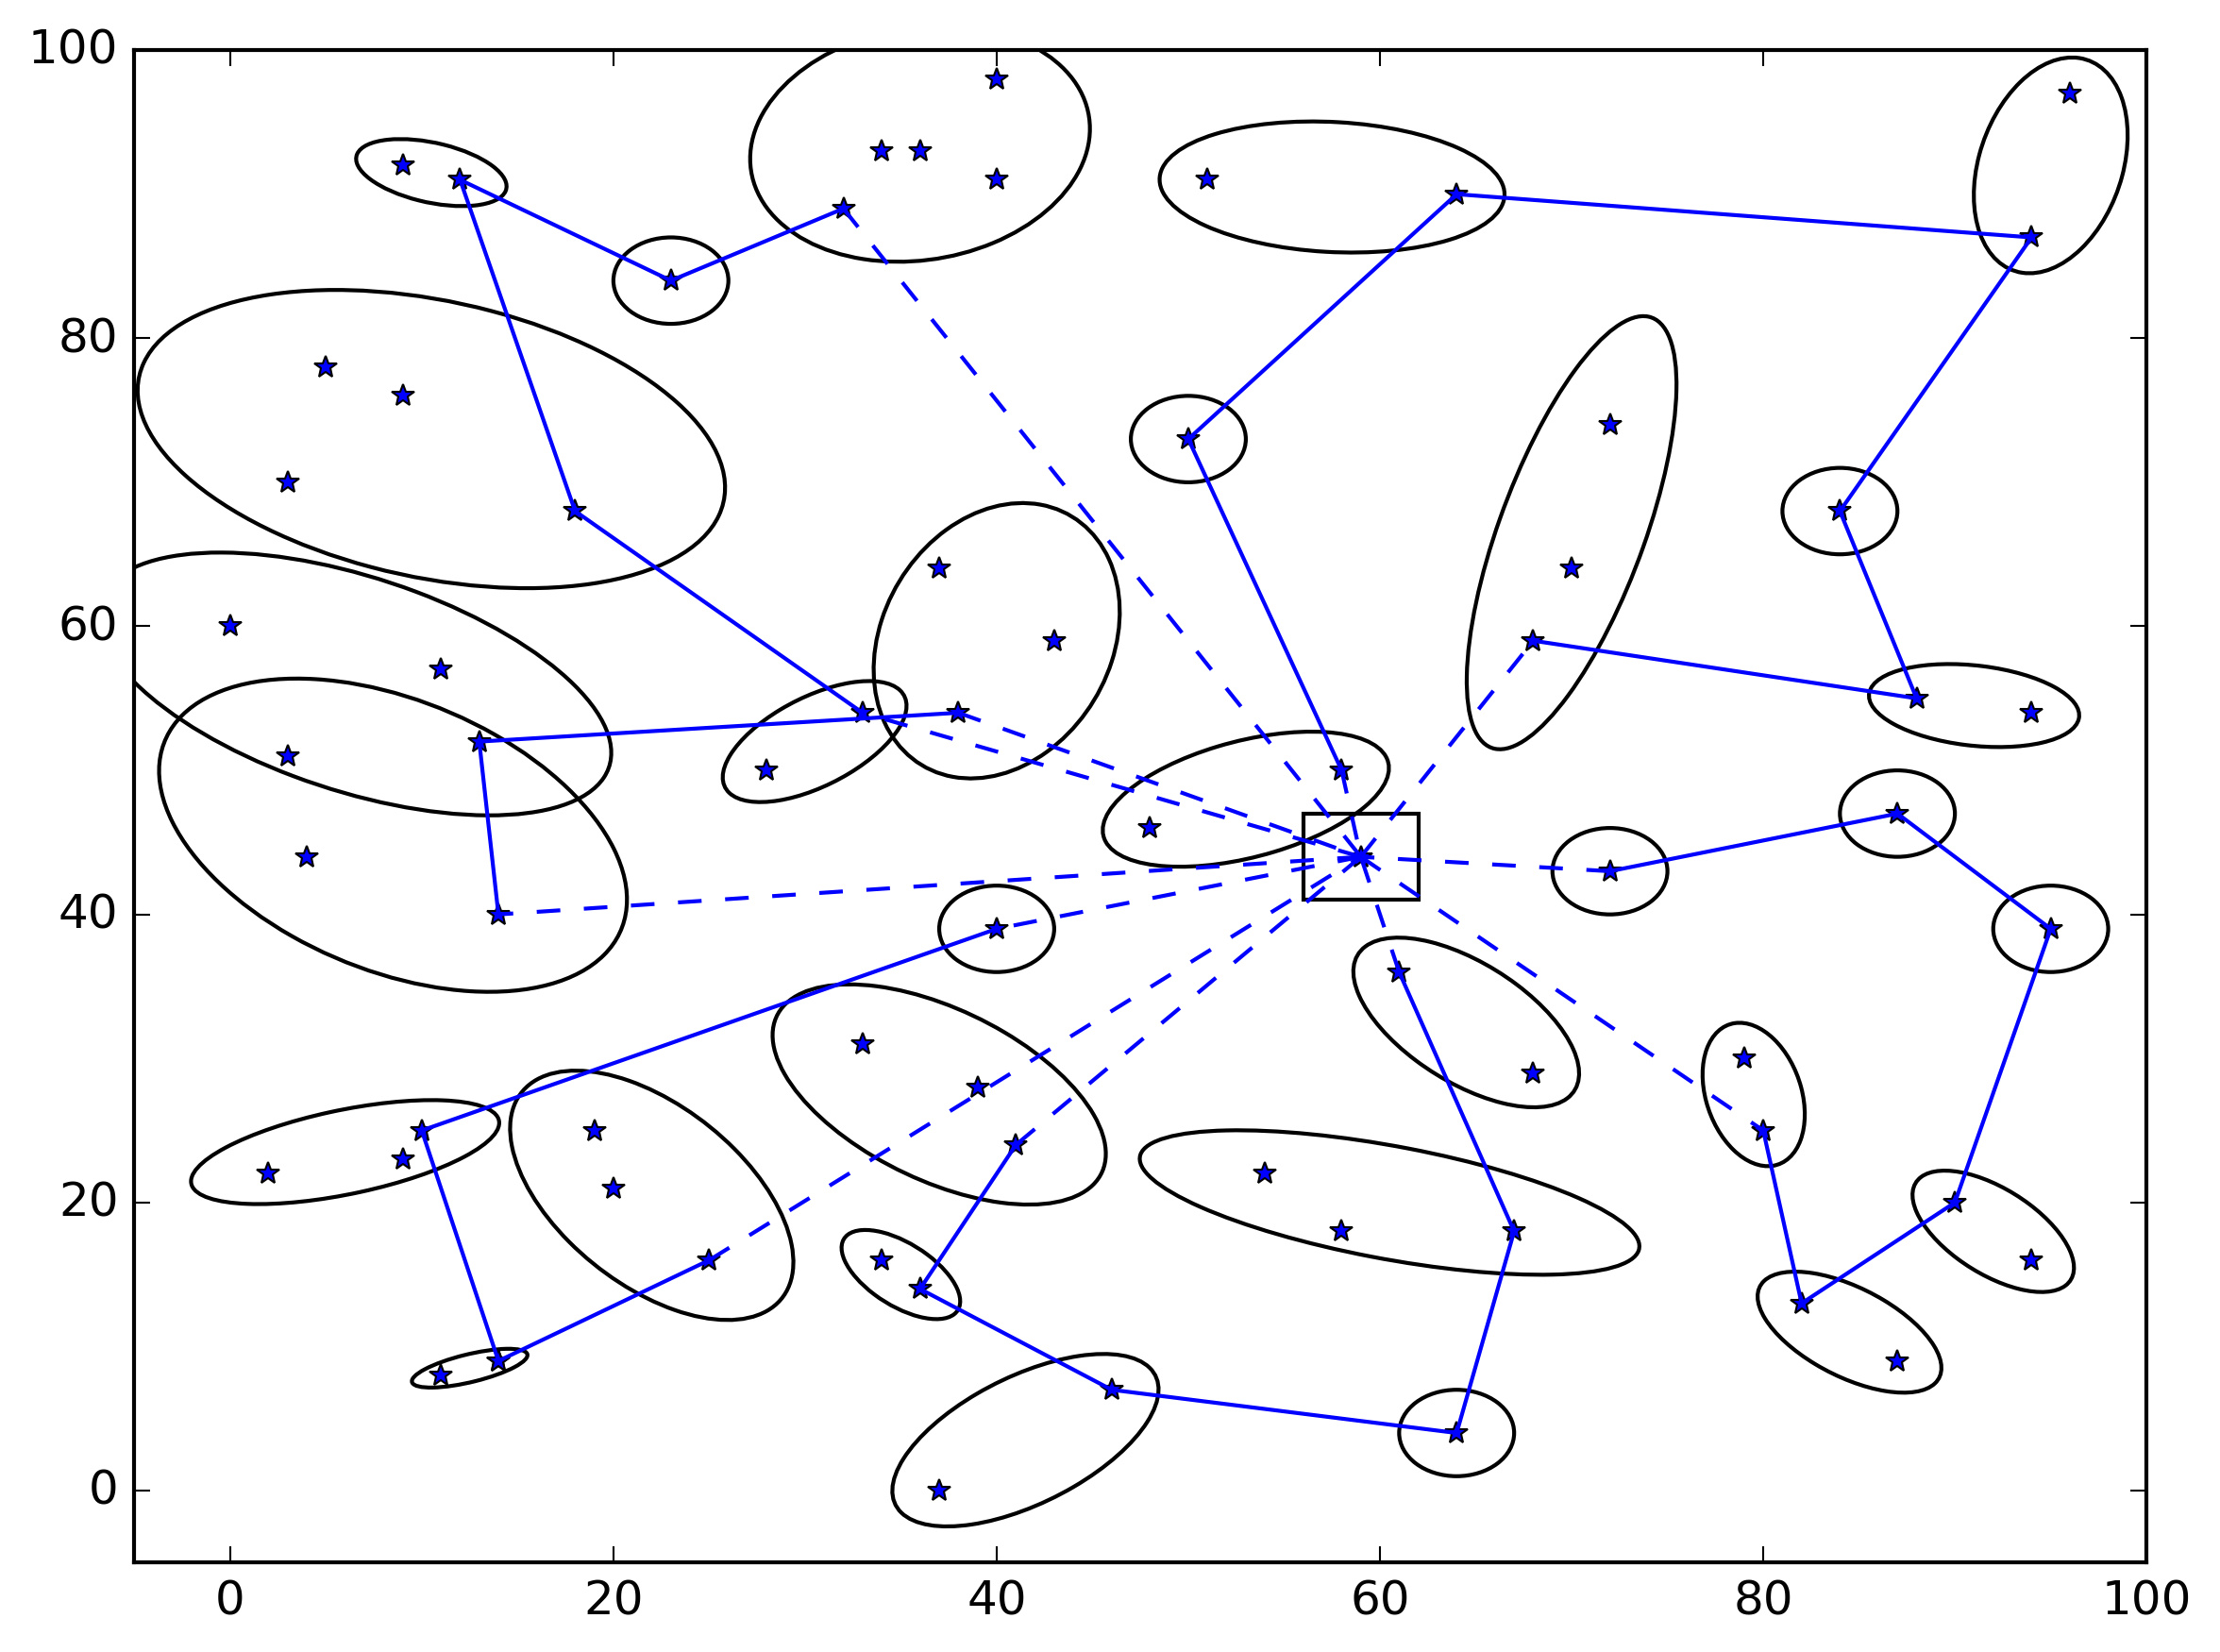
\includegraphics[width=0.45\textwidth]{A-n69-k9-c31_flow_n69_k32_m6_Q150_TL240_map.png}
\label{fig:plots_12}}
\caption{\texttt{A-n69-k9} (clustered)}
\label{fig:A-n69-k9-sol}
\end{figure}

\section{Conclusions}
Two MILP formulations of the generalized vehicle routing problem (GVRP) were studied. The number of variables and constraints is a polynomial function of the number of customers for both the formulations. 
Two formulations were defined: the first had auxiliary variables defined based on the customers (node-based) where as the second had auxiliary variables defined based on arcs between customers (flow-based). 

Three new instances were generated by clustering benchmark instances for the capacitated vehicle routing problem (CVRP). Computational studies were conducted to compare the node-based and flow-based formulations.
The flow-based formulation was proved to have better computational properties as compared to the node-based formulation for all instances under consideration. Two of the new instances were solved to optimality using the superior flow-based formulation. 

\begin{figure}[htbp]
\centering
\subfloat[Customer clusters]{%
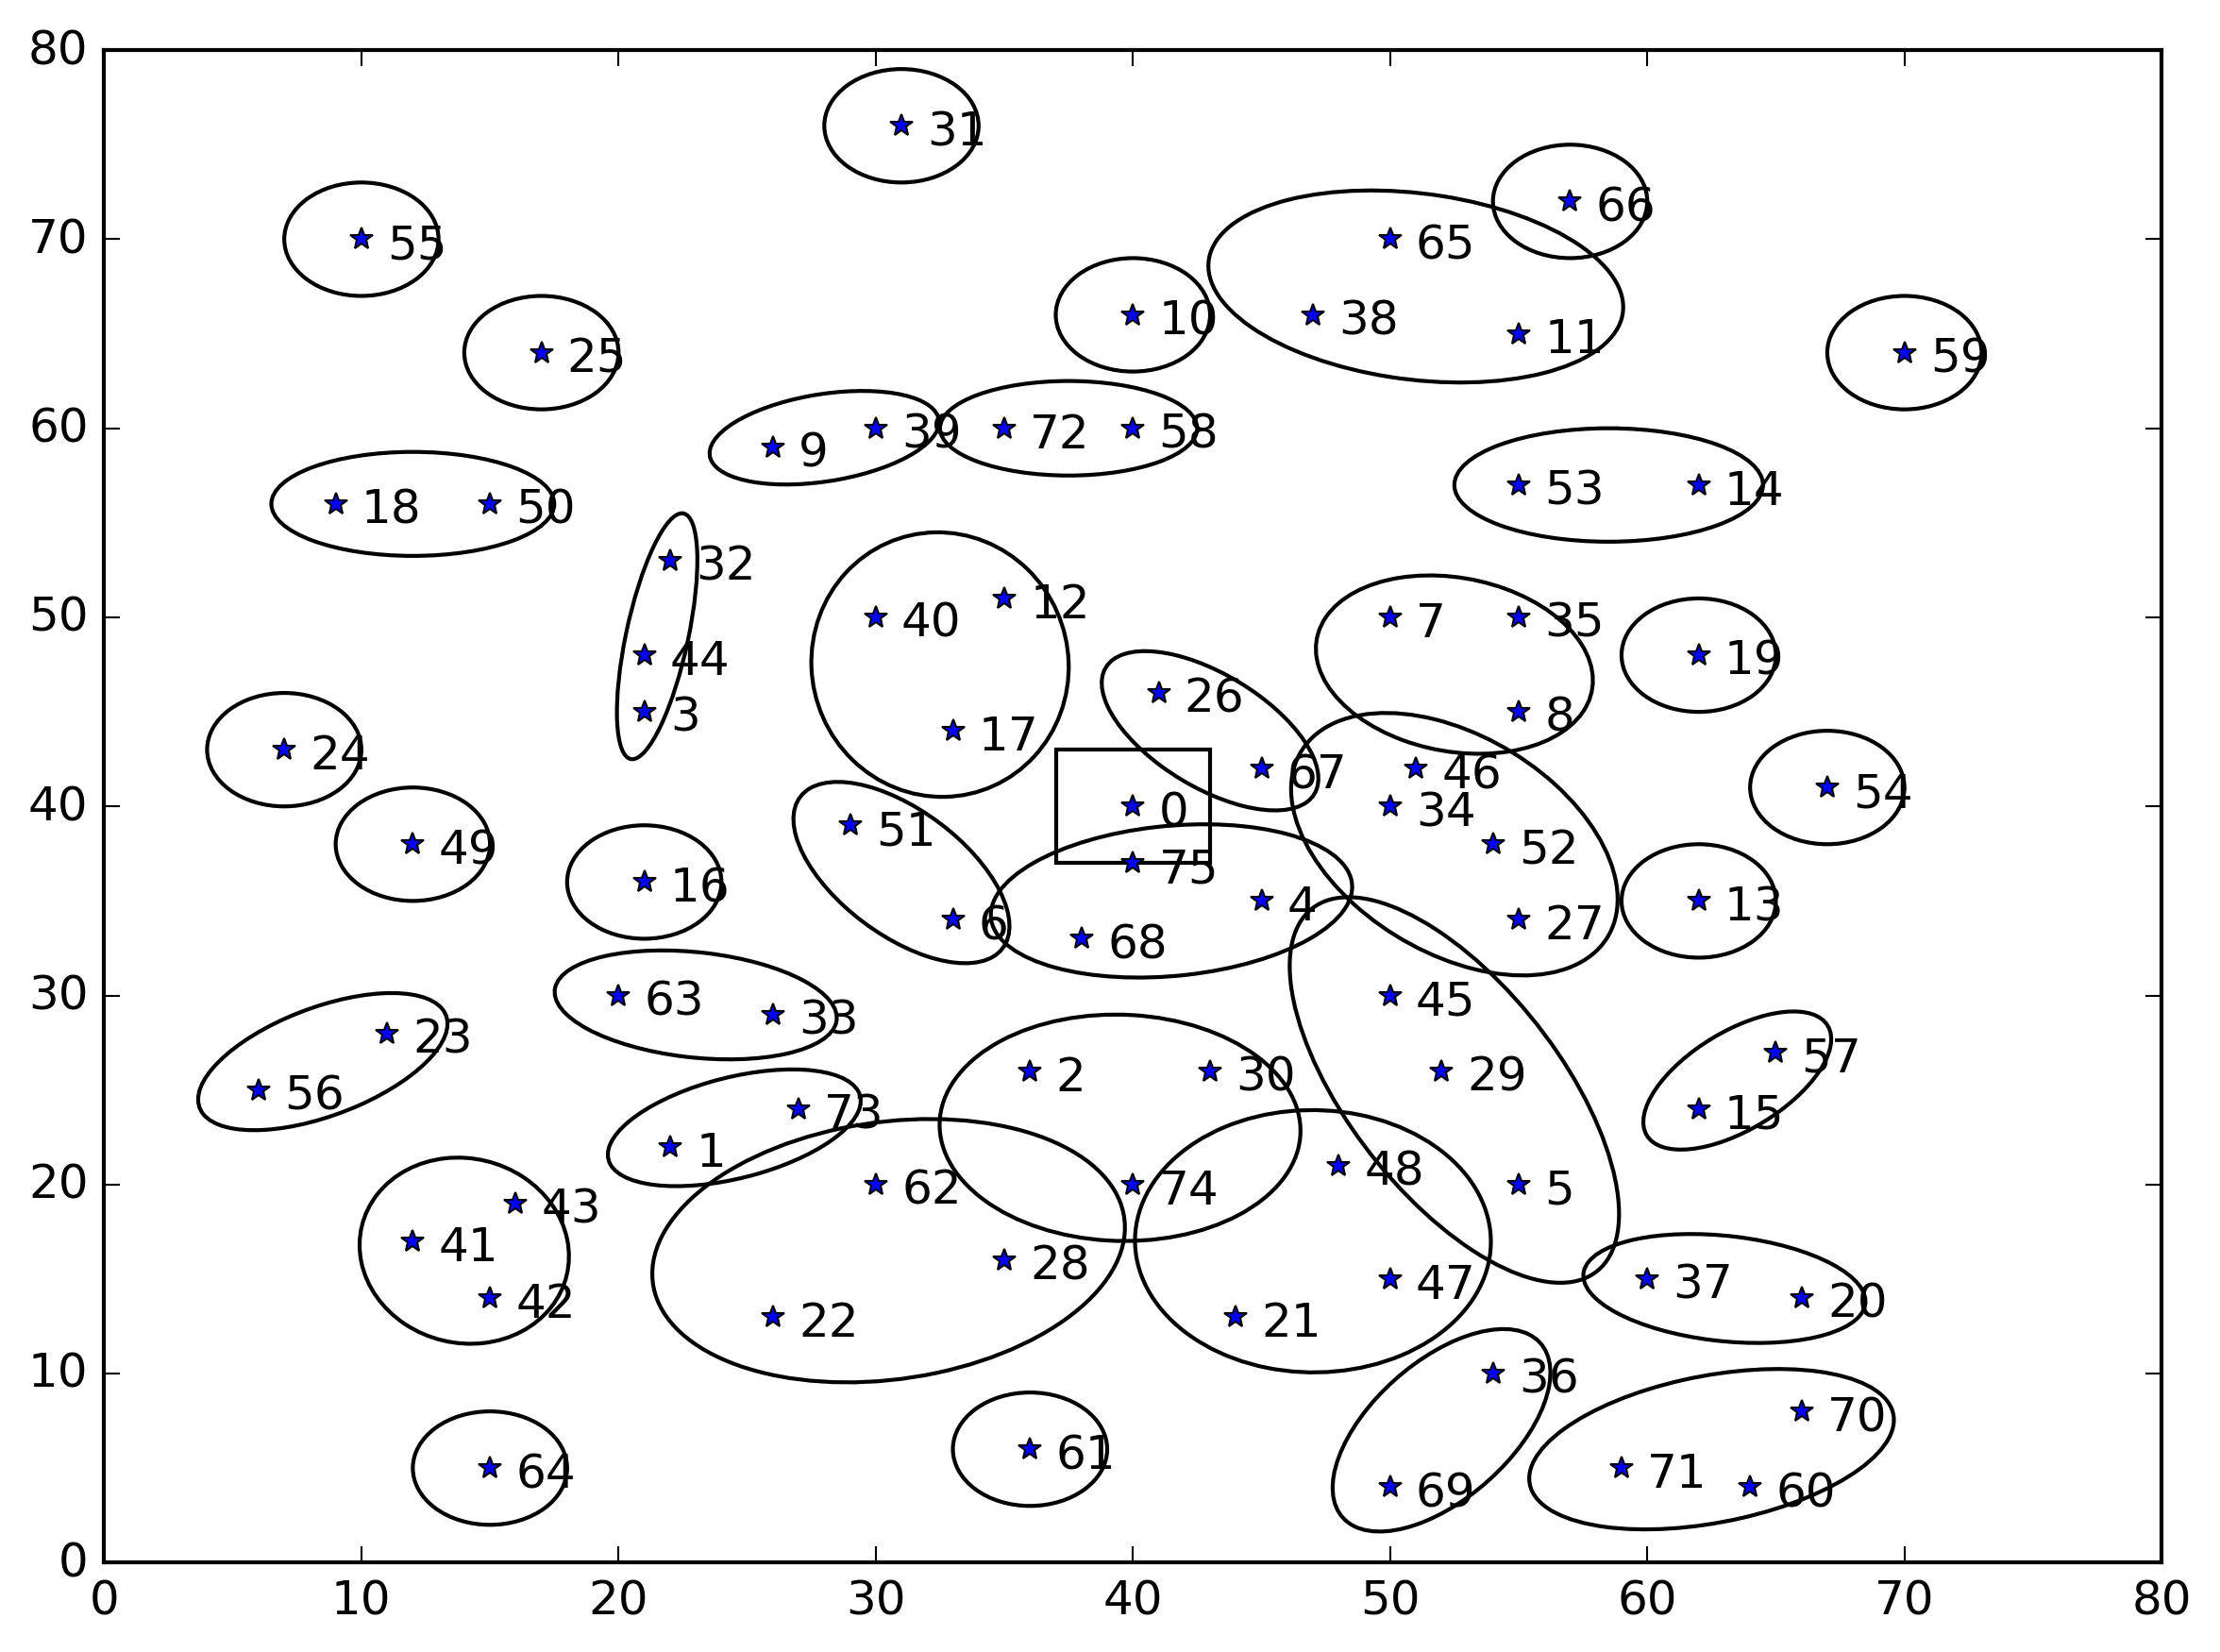
\includegraphics[width=0.45\textwidth]{P-n76-k5-c38_map.png}
\label{fig:plot_11}}
\quad
\subfloat[Best known solution (objective = 500.955)]{%
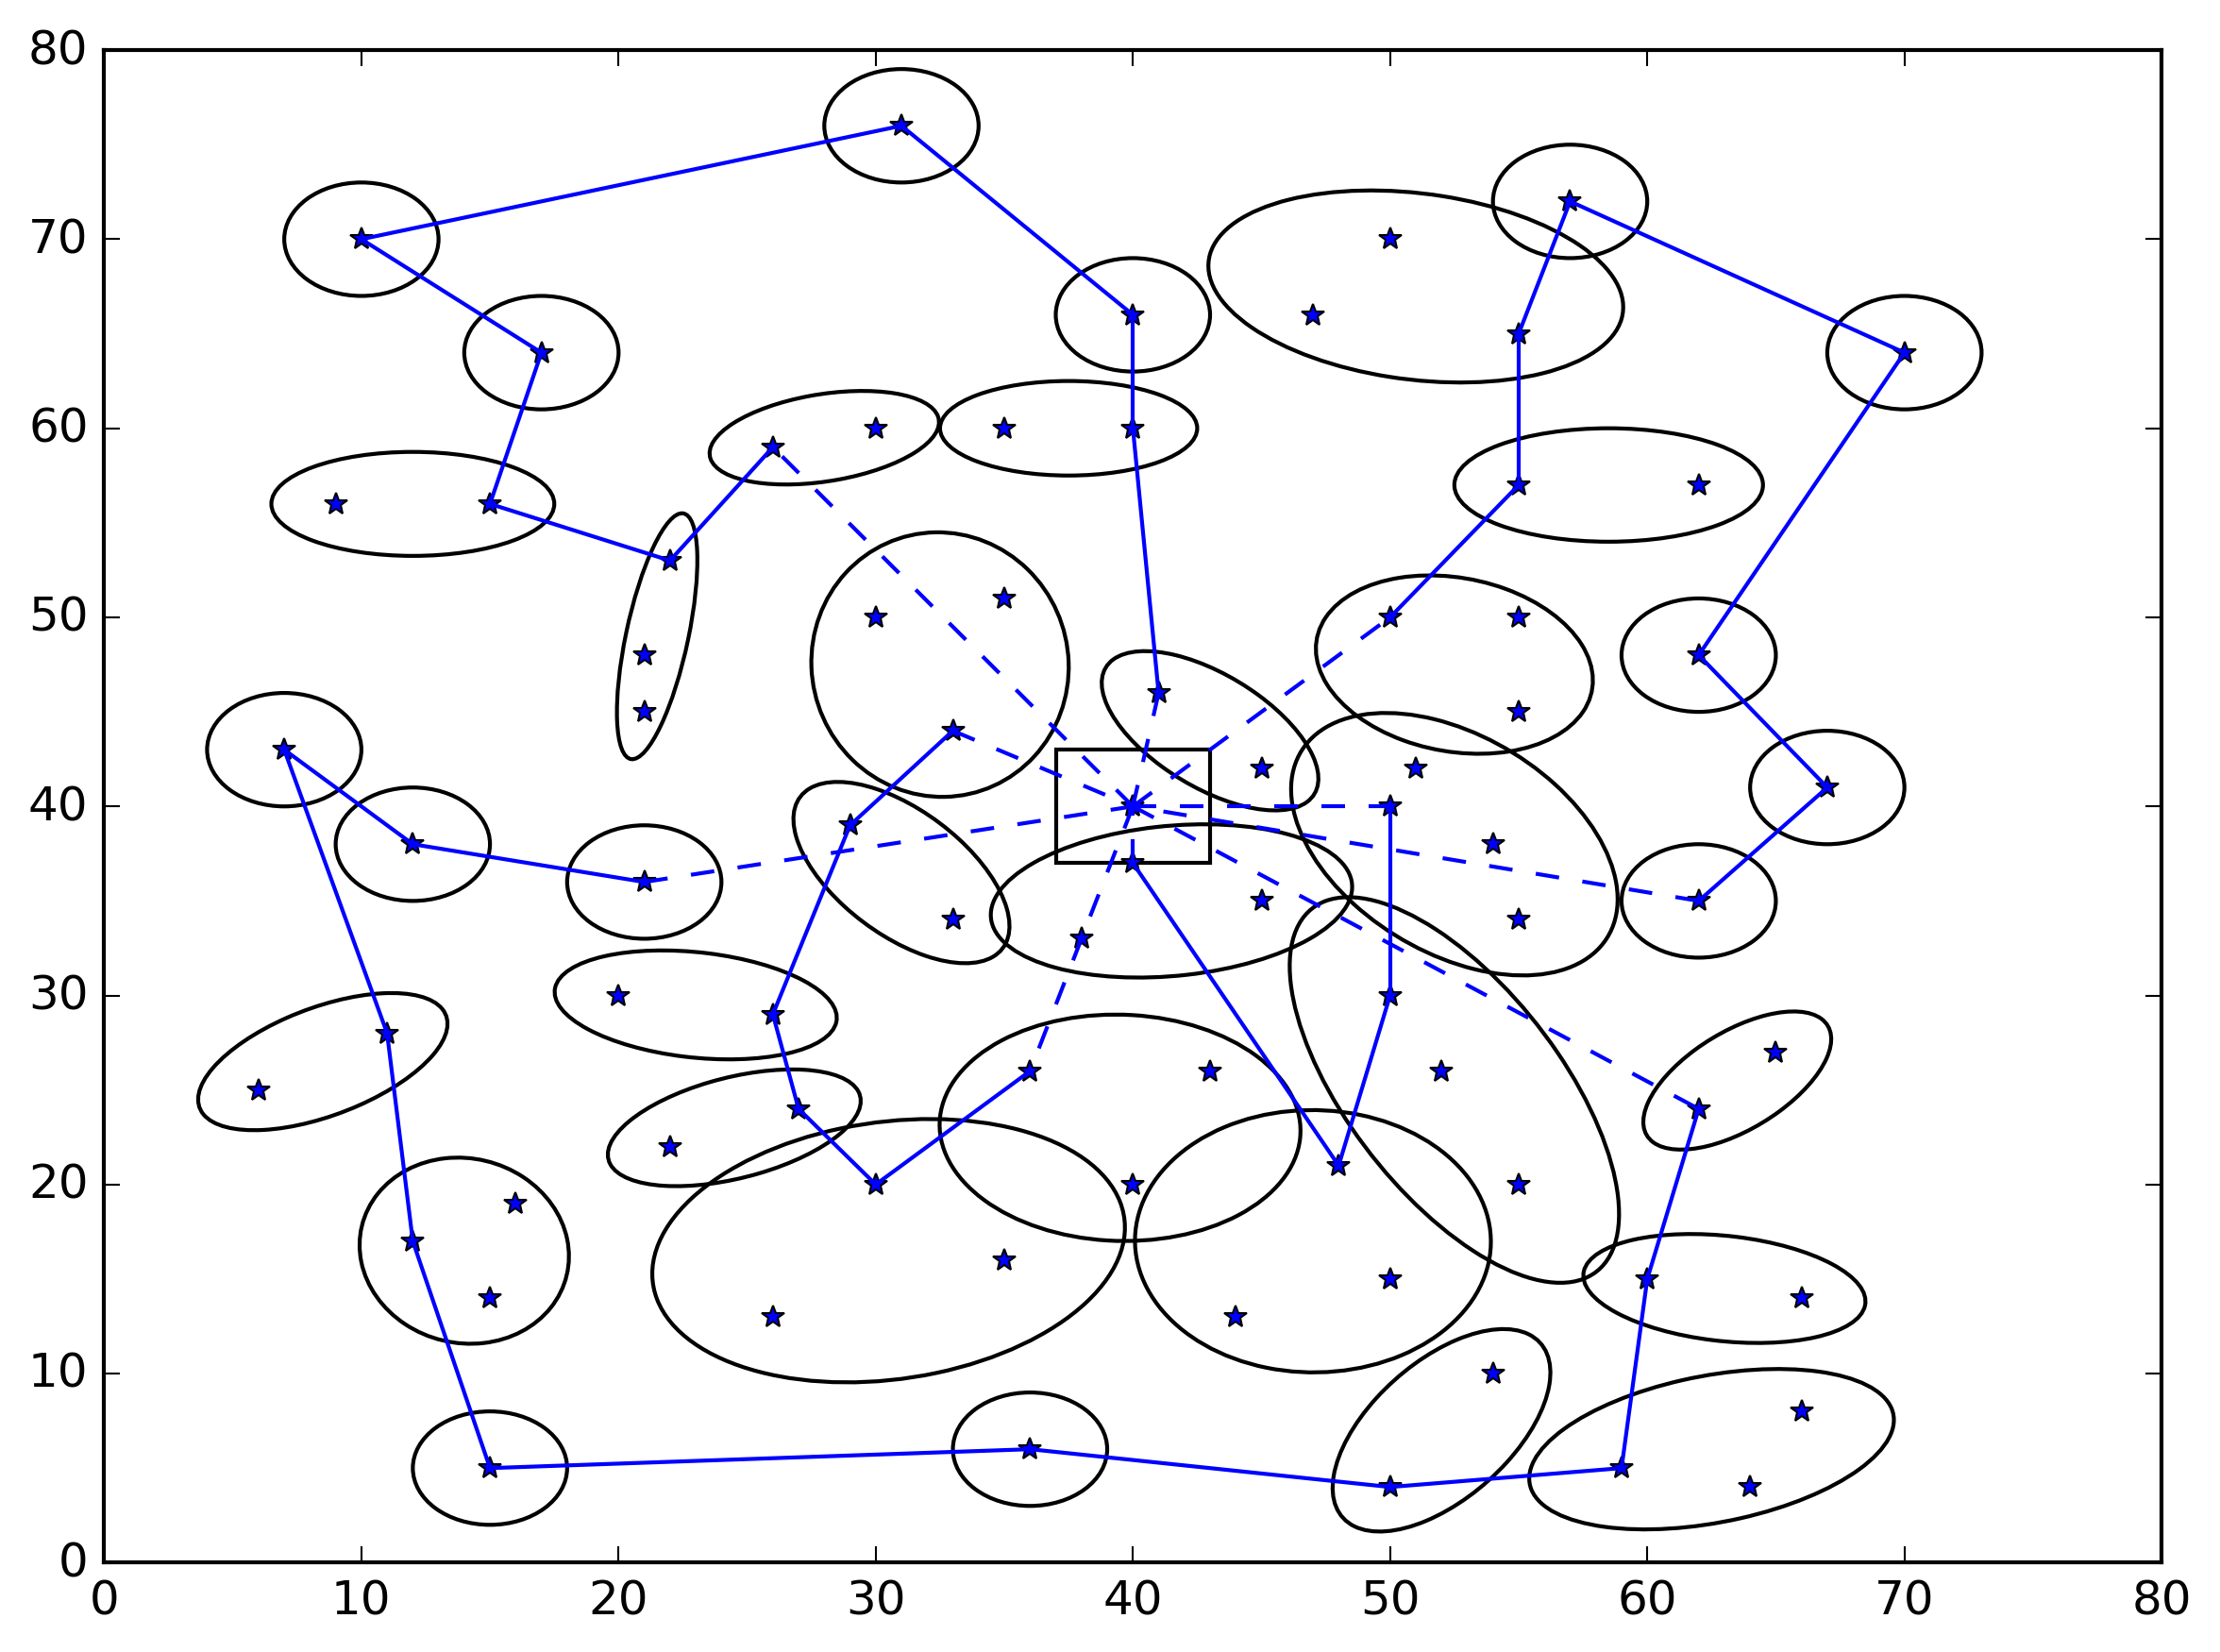
\includegraphics[width=0.45\textwidth]{P-n76-k5-c38_flow_n76_k39_m5_Q280_TL480_map.png}
\label{fig:plots_12}}
\caption{\texttt{P-n76-k5} (clustered)}
\label{fig:P-n76-k5-c38-sol }
\end{figure}

\newpage
%\nocite{*}  %% uncomment to include all references in bib file
\bibliographystyle{ICTv3}
\bibliography{Proposal_bib}

\newpage

%\section*{Appendix}
%
%\renewcommand{\thefigure}{A\arabic{figure}}
%\setcounter{figure}{0}


%\begin{figure}[htbp]
%\centering
%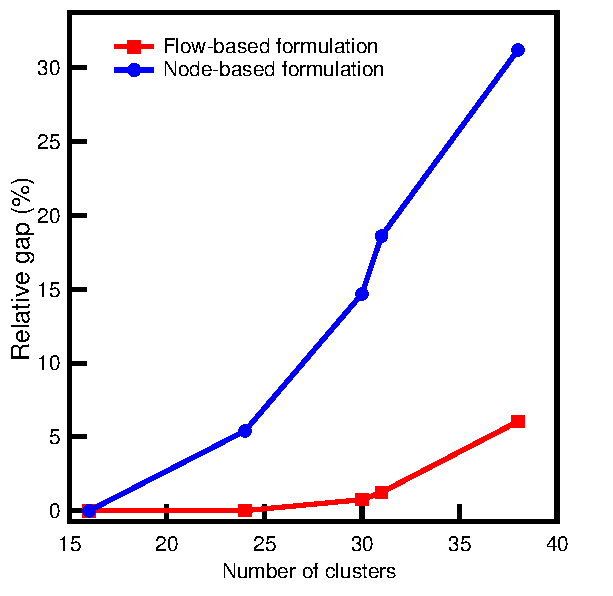
\includegraphics[width=0.6\textwidth]{cok.pdf}
%\caption{asfda}
%\label{fig:w}
%\end{figure}

\end{document}